\documentclass[12pt]{report} %\documentclass[12pt,twocolumn]{report}

\usepackage[T1]{fontenc}
\usepackage[utf8]{inputenc}
\usepackage[hidelinks]{hyperref}
\usepackage{nameref}
\usepackage{amssymb,amsmath, amsthm}
\usepackage{proof-at-the-end}
\usepackage{graphicx,color,soul}
\usepackage[english]{babel}
\usepackage{csquotes}
\usepackage{caption}
\usepackage{subcaption}
\usepackage{multirow}
%\usepackage[square,comma,numbers]{natbib}
\usepackage[style=numeric]{biblatex}
\usepackage{enumitem}
\usepackage{appendix}
\usepackage{fancyhdr}
\pagestyle{fancy}
\setlength{\headheight}{14.5pt}

% Definitions
\theoremstyle{definition}
\newtheorem{defEnd}{Definition}[section]
\newtheorem*{defEnd*}{Definition}
\providecommand*\thmautorefname{Definition}
\newcommand{\adddeftocontentsline}[2]{\addcontentsline{toc}{subsection}{Definition~\ref{#1}. #2}}

% Research Questions
\newtheorem{rqEnd}{Research Question}
\newtheorem*{rqEnd*}{Research Question}
\providecommand*\thmautorefname{Research Question}
\newcommand{\addrqtocontentsline}[1]{\addcontentsline{toc}{subsection}{RQ~\ref{#1}}}

% \usepackage[acronym]{glossaries}
% \makeglossaries
% \newacronym{sba}{SBA}{Segmentation by Annotation}
% \newacronym{dsa}{DSA}{Distance-based Segmentation and Annotation}
% \newacronym{msa}{MSA}{Music Structure Analysis}
% \newacronym{mir}{MIR}{Music Information Retrieval}
% \newacronym{aas}{AAS}{Automatic Audio Segmentation}

% Handy Commands
\newcommand{\sba}{Segmentation by Annotation}
\newcommand{\dsa}{Distance-based Segmentation and Annotation}
\newcommand{\msa}{Music Structure Analysis}
\newcommand{\mir}{Music Information Retrieval}
\newcommand{\aas}{Automatic Audio Segmentation}

% \newcommand{\sba}{\acrlong{sba}}
% \newcommand{\dsa}{\acrlong{dsa}}
% \newcommand{\msa}{\acrlong{msa}}
% \newcommand{\mir}{\acrlong{mir}}
% \newcommand{\aas}{\acrlong{aas}}

%\usepackage[bibliography=common,appendix=append]{apxproof}

\usepackage{mathptmx} % Times new Roman
%\usepackage[a4paper, total={5.4in, 8in}]{geometry}
\usepackage[a4paper, total={5.4in, 9in}]{geometry}

\addbibresource{literature/literature.bib}
\addbibresource{literature/rnn_lstm.bib}
\addbibresource{literature/cnn.bib}

\begin{document}

\begin{titlepage}
    \begin{center}
        \vspace*{1cm}

        \Huge
        \textbf{On Music Structure Analysis}

        \vspace{0.5cm}
        \LARGE
        Machine learning implementations of the Segmentation by Annotation approach

        \vspace{1.5cm}
    \end{center}
    \large
    \textit{Author:}\hfill\textit{Supervisor:} \\
        Leander van Boven\hfill Dr. M.P. (Marijn) Schraagen
        \begin{flushright}
            \textit{Second Supervisor:} \\
            Prof. dr. C.J. (Kees) van Deemter \\
        \end{flushright}

    \vfill
    \begin{center}
        A thesis presented for the degree of\\
        Bachelor of Science

        \vspace{0.8cm}

        \href{https://www.uu.nl/bachelors/kunstmatige-intelligentie}{
\includegraphics[width=0.4\textwidth]{images/uu_logo}}
    
        \Large
        Faculty of Humanities\\
        University Utrecht\\
        The Netherlands\\
        June 2020
    \end{center}
\end{titlepage}

\thispagestyle{plain}
\begin{center}
    \Large
    \textbf{On Music Structure Analysis}

    \vspace{0.4cm}
    \large
    Machine learning implementations of the Segmentation by Annotation approach

    \vspace{0.4cm}
    \textbf{Leander van Boven (6215637)}

    \vspace{0.9cm}
    \textbf{Abstract}
\end{center}
This thesis proposes a novel approach to Music Structure Analysis (MSA). This approach implements the Segmentation by Annotation (SbA) approach to MSA, using a convolutional neural network (CNN) and an artificial neural network using Long Short-Term Memory (LSTM) units. An overview of the current advances in music structure analysis is given as well as the use of the proposed architectures in similar research fields. A description of the testing methods is provided in which the proposed architectures show promising results on the custom ground truth used. This custom ground truth is a modified version of the segment function annotations found in the internet archives subset of the SALAMI dataset. The ground truth is modified by reducing the amount of unique functions from 26 to 9 because of the low occurrence of some labels in the original data and to improve the accuracy of the machine learning models. Due to this custom ground truth, comparison with the current state-of-the-art of music structure analysis proved quite hard. By comparing the SbA approach to the (more symbolic) Distance-based Segmentation and Annotation approach, a comparison between using machine learning and non-machine learning techniques can be made. Future research is proposed to enhance the segmentation by annotation approach as well as music structure analysis in general.\\
\\
\textbf{Keywords:} Music Structure Analysis, Music Information Retrieval, Segmentation by Annotation, Convolutional Neural Networks, Long Short-Term Memory

\clearpage

\thispagestyle{empty}
\null\vfill

\newlength\longest
\settowidth\longest{\large\itshape The more we think we know about, the greater the unknown}
\begin{center}
    \parbox{\longest}{%
    \raggedright{\large\itshape%

    %More things than are dreamed about, unseen and unexplained\\
    %We suspend our disbelief, and we are entertained\\
    The more we think we know about, the greater the unknown\\
    We suspend our disbelief, and we are not alone\\
    Mystic rhythms -- capture my thoughts\\
    Carry them away\dots\\
    \par\bigskip
    }   
    \raggedleft\large\MakeUppercase{Neil Ellwood Peart}\\\small Rush - Mystic Rhythms\par%
    }
\end{center}

\vfill\vfill

\clearpage


\tableofcontents

\chapter{Introduction}
\label{ch:intro}
Music is all around us. Everybody listens to it in a different way \cite{Cox2012a}, only a few actually create it. Creating music takes a lot of effort; making sure all notes and tones form some kind of harmony and melody, and that all harmonies and melodies form a coherent piece, among many other difficult aspects that involve creating music. Although these aspects are all very difficult and only some people are actually good at it, computers are far worse in it.\\
Listening to music involves many subconscious processes that are influenced by, among other things, emotion. Therefore making a computer understand the concept of music is a difficult task.
Due to the hierarchical properties of music \cite{Cooper1960rhythmic, Lerdahl1983overview}, one of the first steps of this process is understanding the musical structure of a piece of music. This will be the main focus of this thesis.


\section{Musical Structure}
The musical structure of a piece of music can be defined in many different ways; on a high level or low level, and can be of different meanings in different kinds of music.\\
Therefore for the remainder of this thesis I will refer to music as music in the genre of Western Popular Music \cite{Serra2012measuring} and make the following definitions:

\theoremstyle{definition}
\adddeftocontentsline{def:musical_structure}{Musical Structure}
\begin{theoremEnd}[restate,category=def]{defEnd}[Musical Structure]
    \label{def:musical_structure}
    The \textit{Musical Structure} of a piece of music is a series of \textit{segments} (\ref{def:segment}) that describes the high-level structure of a piece of music.
\end{theoremEnd}

\adddeftocontentsline{def:segment}{Segment}
\begin{theoremEnd}[restate,category=def]{defEnd}[Segment]
    \label{def:segment}
    A \textit{Segment} is one consecutive piece of audio in a piece of music that has one \textit{segment function} (\ref{def:segment_function}), with a start- and an end-boundary.
\end{theoremEnd}

\adddeftocontentsline{def:segment_function}{Segment Function}
\begin{theoremEnd}[restate,category=def]{defEnd}[Segment Function]
    \label{def:segment_function}
    Following the definitions as they can be found in \textcite{Benward1997music}, Part B: \textit{The Structural Elements of Music}, a \textit{Segment Function} is the function of a \textit{segment}, this is either:
    \begin{itemize}[noitemsep]
        \item Chorus
        \item Verse
        \item Bridge
        \item Interlude / Transition
        \item Intro
        \item Outro
        \item Solo
        \item (Silence)
        \item (Background Noise)
    \end{itemize}
\end{theoremEnd}

I will refer to the extraction of the musical structure of a piece of music as \textit{Musical Structure Analysis} or MSA. An example of musical structures can be found in \autoref{fig:music_structures_examples}. The aim of this thesis is to produce a structure of a song similar to \ref{fig:music_structures_examples}e and \ref{fig:music_structures_examples}f, where \textbf{I} stands for intro, \textbf{V1} stands for Verse 1, etc.

\begin{figure}[t]
    \centering
    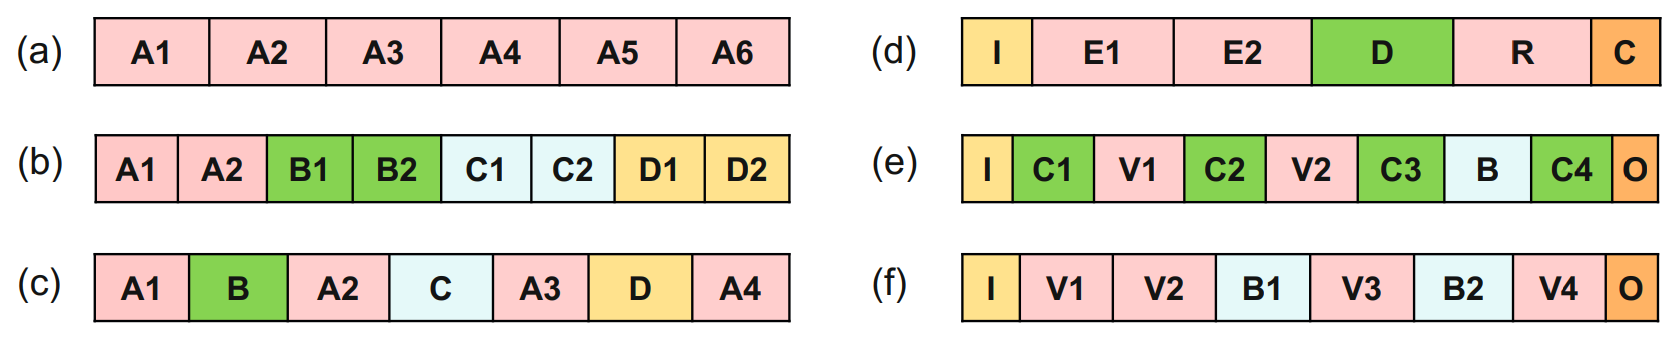
\includegraphics[width=1\textwidth]{images/music_structures_examples}
    \caption{Examples for musical structures as encountered in Western music. \textbf{(a)} Strophic form. \textbf{(b)} Chain form with repetitions. \textbf{(c)} Rondo form. \textbf{(d)} Sonata form. \textbf{(e)} Beatles song “Tell Me Why.” \textbf{(f)} Beatles song “Yesterday.”\\
    Reprinted from \textcite[p. 173]{Muller} (Figure 4.4)}
    \label{fig:music_structures_examples}
\end{figure}


\section{Applications}
The musical structure of a piece of music has many applications, within research and the industry. For example the musical structure can be used to only retrieve a certain part of a piece of music. This can then be used to preview only the chorus of a song when someone is browsing through a list of songs to find a certain song. Being able to quickly seek through a song to its verses or chorus can be of great addition to many music streaming, or other streaming, services. 

More commercial applications could be to limit ones listening capabilities by restricting a user to listen only to the verse or chorus of a song, while blocking the other parts of a song behind some pay-wall. Less aggressive commercial applications could be to place an advert between for example the verse and chorus, when the user is using a free subscription to a music streaming service.

The scope of this thesis, however, will be to place the music structure problem in a more research driven, less commercial field, and the field of AI in particular.

\subsection{Relevance to AI}
Finding and analyzing the structure of a musical piece is an important part of music information retrieval and an important step in music processing and music analysis, both for humans and computers. Once an understanding of the basic structure of a piece of music is established, it can be used to establish more complex understandings about that piece of music.

One of these uses may be to use the musical structure to get more insight in how certain songs are equal to each other, or how certain structures are used for certain kinds of songs or in certain genres. This thus may be used as additional information when finding for example the genre of a piece of music.

Another way of using this musical structure could be to extract lower level musical patterns from a piece of music. This could be leading melodies, a riff\footnote{A famous example of a (rock) riff can be found in \textit{Smoke on the Water} played by Ritchie Blackmore of Deep Purple.}, lyrics or the hook \cite{Covach2005form} of a song \cite{Chai2005automated}.

Additionally, knowledge about the structure of songs that are produced by humans can be used for generating songs using computers. This information can for example be used as additional information during the generation phase, or as validation information for already generated songs to validate whether these generated songs comply to human musical structure.\\

For humans, finding the musical structure is quite trivial, because they constantly and often unconsciously adapt themselves to the musical and acoustic properties of what they listen to. However the amount of different musical structures make computational structure analysis a challenging problem.


\section[SbA vs DSA]{\sba\ versus\\ \dsa}
Extracting the musical structure of a piece of music can be done in a few ways, however almost all of these methods can be generalized into two general approaches: \textit{\sba}\ (SbA) and \textit{\dsa} (DSA).

\adddeftocontentsline{def:SbA}{\sba}
\begin{theoremEnd}[restate,category=def]{defEnd}[\sba]
    \label{def:SbA}
    \textbf{\sba} in the context of music structure analysis means first dividing a song into many small pieces (e.g. pieces of 10ms or every beat). Thereafter a \textit{segment function} is assigned to each small piece using some kind of classification method (e.g. statistics, support vector machine, deep learning). Sequences of similarly annotated small pieces are then combined into \textit{segments}, resulting in the musical structure of the song.
\end{theoremEnd}

\adddeftocontentsline{def:DSA}{\dsa}
\begin{theoremEnd}[restate,category=def]{defEnd}[\dsa]
    \label{def:DSA}
    \textbf{\dsa} in the context of music structure analysis means first finding segment boundaries using some kind of distance metric. Subsequently these segments are grouped into groups that are similar to each other in their structural role in the piece of music, using some kind of grouping method (e.g. nearest neighbors, support vector machines), resulting in each segment getting a capital letter denoting their function. Then, each capital letter is converted into a segment function, this can be either done using some kind of statistics, pattern matching or machine learning method.
\end{theoremEnd} 

\dsa\ has been researched a lot in the context of music structure analysis and was for a long time the best approach. See \autoref{ch:r_work} for an overview of research in this areas. \sba\ has been used a lot less for this exact application but more for separating and classifying pieces of speech, music and different kind of background noises in an audio stream. This is because speech, music and background noise all differ a lot more in their auditory features than different parts of music within the same piece. Because the use of the distance-based approach yielded increasingly better results, recent research focused on that. However with the increasing popularity and performance of machine learning in many disciplines like computer vision or natural language processing and production, applying machine learning to the music structure problem has become increasingly popular.


\section{Combined Research}
Although the DSA approach to MSA is become state-of-the-art, its results can always be improved. Therefore not only putting effort into improving the \sba\ approach but also the \dsa\ approach will benefit the \msa\ problem. This work is related to \textcite{Jesperthesis} in such a way that this work focuses on the \sba\ approach, and \citeauthor{Jesperthesis} focuses on giving an overview and improvement of the \dsa\ approach.


\section{Research Questions}
The following research questions can be formulated:

\addrqtocontentsline{rq:main}
\begin{theoremEnd}[restate,category=rq]{rqEnd}[Main RQ]
    \label{rq:main}
    What is the feasibility of a machine learning implementation of the \sba\ approach to \msa\ in Western Popular Music?
\end{theoremEnd}

The sub-questions that are part of this main research question are:

\addrqtocontentsline{rq:sub1}
\begin{theoremEnd}[restate,category=rq]{rqEnd}[Sub-RQ 1]
    \label{rq:sub1}
    Which deep learning architecture, implementing the \sba\ approach to \msa, yields the best relative results?
\end{theoremEnd}

\addrqtocontentsline{rq:sub2}
\begin{theoremEnd}[restate,category=rq]{rqEnd}[Sub-RQ 2]
    \label{rq:sub2}
    How does the performance of the best performing deep learning architecture, implementing the \sba\ approach to \msa, compare to the performance of implementations of the \dsa\ approach, and a state-of-the-art implementation in particular?
\end{theoremEnd}

To answer the main research question I will create different types of deep learning models, using different kinds of architectures. Then I will train these models on different combinations of musical features extracted from the songs present in the internet archives subset of the SALAMI dataset (see \autoref{sec:3.the_data} for an explanation of this dataset). I will use the annotations, produced by human annotators, of these songs as ground truth to determine the absolute performance of each implementation. The absolute performance of the best performing implementation can then be used to compare a machine learning application of the \sba\ approach to MSA to the absolute performance of a state-of-the-art implementation of the \dsa\ approach, determined in the same way. I will elaborate more on this in \autoref{ch:method}.


\section{Outline}
In \autoref{ch:r_work} I will first explore previous work regarding the SbA and DSA approach. Here I will also discuss the current state-of-the-art and describe the background of the models I created. Lastly I will give an overview of the dataset I used, and a listing of possible acoustic features that can be extracted from this dataset.

In \autoref{ch:method} I introduce the architectures of the models I created. In this chapter I also describe the data preparation and feature selection that preceded the testing phase of this research.

Then, in \autoref{ch:results} I describe the training and evaluation setup and some preliminary results. A final test setup is described as well as the final results following from this final test.

Thereafter, \autoref{ch:discussion} discusses these results and explores reasons for these results. It concludes with a comparison between the segmentation by annotation approach and distance-based segmentation and annotation approach to music structure analysis.

This thesis ends with \autoref{ch:future_research}. In this final chapter I propose future research that can be performed to improve both the segmentation by annotation approach to music structure analysis as well as music structure analysis in general. This chapter ends with an comparison of machine learning versus symbolic approaches to music structure analysis as well as artificial intelligence problems in general.

\chapter{Related Work}
\label{ch:r_work}
In this chapter I will give an overview of applications within branches of music information retrieval that are related to music structure analysis. Two machine learning architectures are introduced. Then previous work of the distance-based segmentation and annotation approach is reviewed and the current state-of-the-art to music structure analysis is showed. This chapter ends with an overview of datasets and acoustic features that can be used for music structure analysis. 


\section[ML in MIR]{Machine learning in Music Information\\Retrieval}
Although machine learning has not been applied on a wide scale to the SbA approach to \msa, it is already being used and researched upon within \mir\ (MIR) and music generation. Because \mir\ involves many disciplines regarding music that extend well beyond the scope of this thesis, as does music generation, I will focus on applications of machine learning closely related to \msa. See \citetitle{Muller} \cite{Muller} for an extensive introduction to basis and main disciplines of \mir.

\subsection[ML for AAS]{Machine Learning for \aas}
\begin{figure}[t]
    \centering
    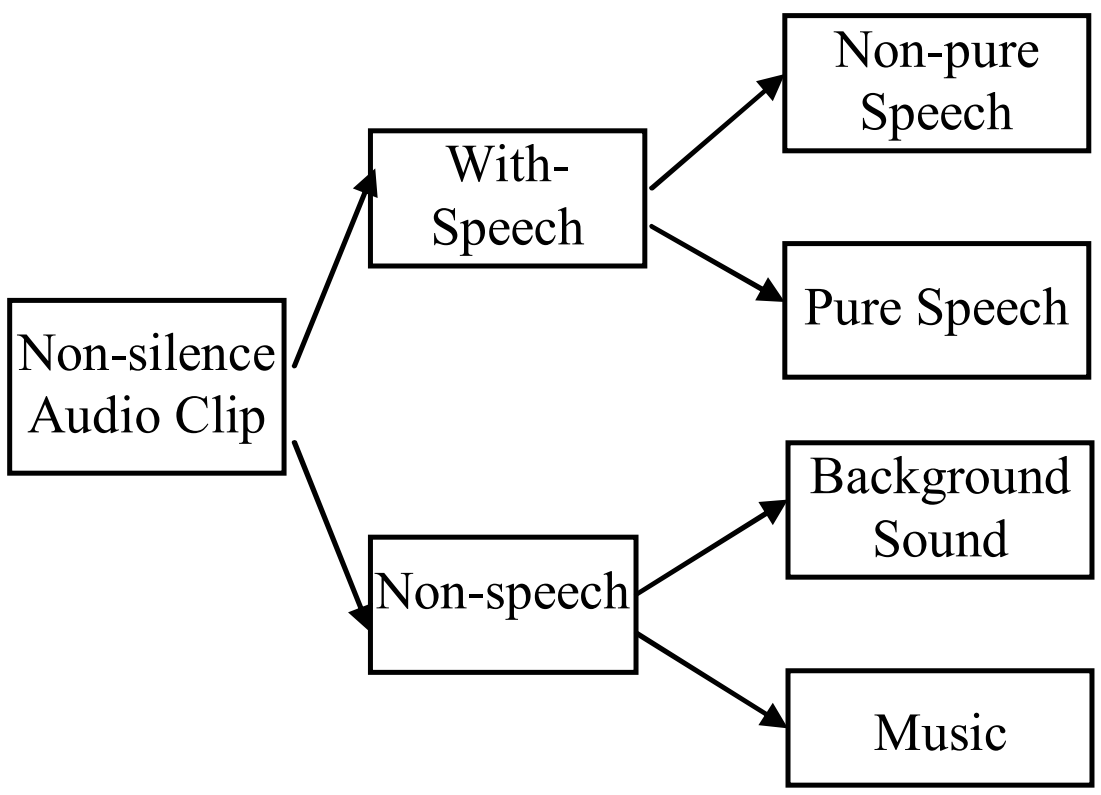
\includegraphics[width=0.5\textwidth]{images/broadcast_classification}
    \caption{Example multi-class classification tree for multi-class broadcast domain data classification or \textit{Automatic Audio Segmentation}.\\
    Reprinted from \textcite{Lu2001content} (Figure 2)}
    \label{fig:broadcast_classification}
\end{figure}
One of the fields in which machine learning has been (successfully) applied, is classifying pieces of audio in an audio stream. The classes to be distinguished are \textit{speech}, \textit{music} and various kinds of \textit{background noises} or \textit{silence}. Each class can be made as specific as desired; one could be interested in finding only the parts within an audio stream where the same person is talking, or where only music is played. This is often referred to as \textit{Automatic Audio Segmentation} (AAS). 

\textcite{Theodorou2014overview} gives an overview of different approaches and implementations to automatic audio segmentation. They describe a distance-based approach similar to the distance-based segmentation and annotation approach to MSA. One of the downsides of this approach is that it does not classify each segment, because it is limited to solely finding the segment boundaries. One other approach they describe is the \sba\ approach. Within automatic audio segmentation, this approach works in a similar way as the SbA approach to music structure analysis, by subdividing an audio stream into small pieces and assigning a class to each small piece. \citeauthor{Theodorou2014overview} mention this approach as being specifically suited for machine learning, because of the high performance of machine learning models on classification problems.

First uses of machine learning used for automatic audio segmentation used machine learning methods that did not employ deep learning, such as Gaussian Mixture Models \cite{Misra2012speech,Kos2009line,Zhang2010audio,Butko2011audio,Dogan2009content}, Support Vector Machines \cite{Richard2007combined,Lu2001content,Zahid2015optimized,Dogan2009content,Patsis2008speech,Lo2010homogeneous} or Decision Trees \cite{Patsis2008speech,Butko2011audio}, often combined into a hybrid model with a Hidden Markov Model.

The main idea of these models is to first make a distinction between \textit{speech} and \textit{non-speech} using a certain classification model and than use other classification models to make further distinctions within speech like \textit{pure speech} or \textit{silence} and non-speech like \textit{pure music} or \textit{background noise} (\autoref{fig:broadcast_classification}). The Hidden Markov Model in this context is used to combine the output of multiple models trained on different labels and assign the final label to the audio sample.\\

 A recent report of more advanced machine learning methods, such as deep learning, being used within \aas\ is from \textcite{Gimeno2020a}. They describe an implementation of the SbA approach to automatic audio segmentation using a recurrent neural network, namely bi-directional long short-term memory artificial neural networks. Their aim was to make use of this architecture with multiple different configurations to find the best model. These different configurations consisted of different pooling layers between multiple long short-term memory layers and different input feature combinations.

\subsubsection{Recurrent Neural Networks}
\begin{figure}[t]
    \centering
    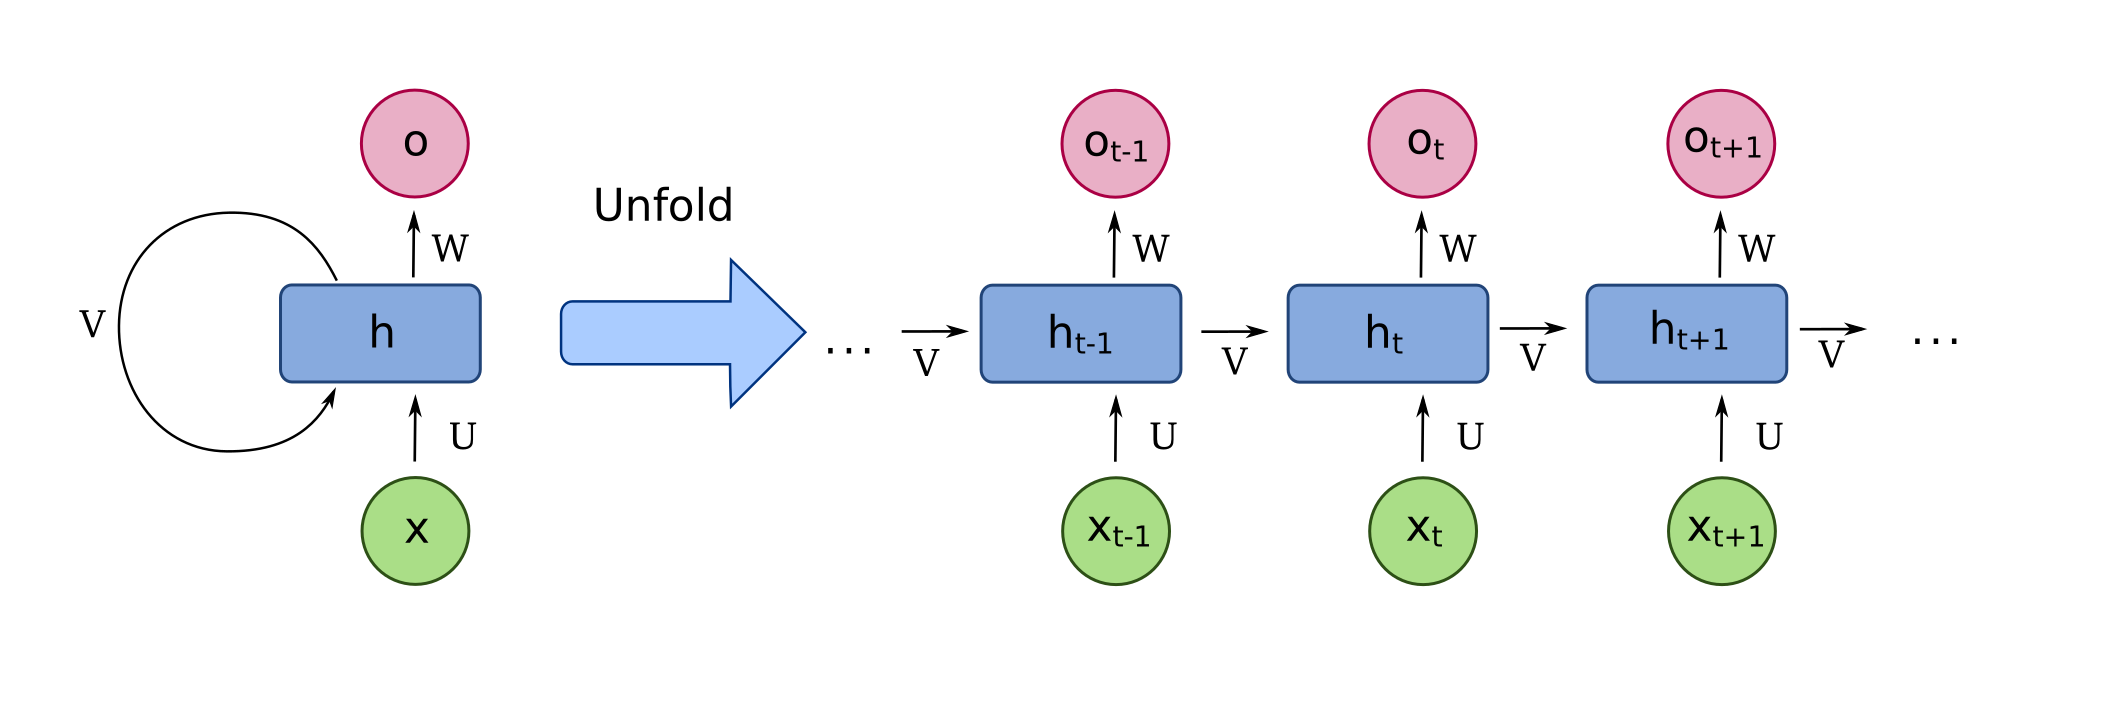
\includegraphics[width=1\textwidth]{images/fully_rnn.png}
    \caption{Basic structure of a fully recurrent neural network.}
    \label{fig:fully_rnn_example}
\end{figure}
A recurrent neural network (RNN) was used because of its capabilities in processing temporal sequence data. This is because this type of artificial neural network has a recurrent architecture, meaning that the output of the previous sample is combined with the input of the current sample \cite{Dupond2019thorough}. The connections of the neurons can be compared to a directed graph. Due to this connectivity, the internal state of the network at a certain point in its training or inference phase can be called memory, because of the still existing output of the previous sample. However, a downside of this architecture is that the previous sample is very present in the 'memory' while earlier samples are increasingly less present. These fully recurrent neural networks therefore have very good short term memory while lacking long term memory (figure \ref{fig:fully_rnn_example}).

Back-propagation (the algorithm used to train artificial neural networks) now has to be performed over time, this is called back-propagation through time (BPTT) \cite{Hochreiter1997long,Robinson1987utility,Werbos1988generalization}. This means that the output of each time step needs to be tracked, which can become quite unwieldy. \textcite{Elman1990finding} found a way around this problem by truncating an unfolded fully RNN to just one time step. This way normal back-propagation can be used again for time sequence data. Elman networks are therefore also called simple recurrent (neural) networks (SRNN). Another type of SRN are Jordan networks \cite{Jordan1997serial}.\\

\subsubsection{(Bi-directional) Long Short-Term Memory Networks}
\begin{figure}[t]
    \centering
    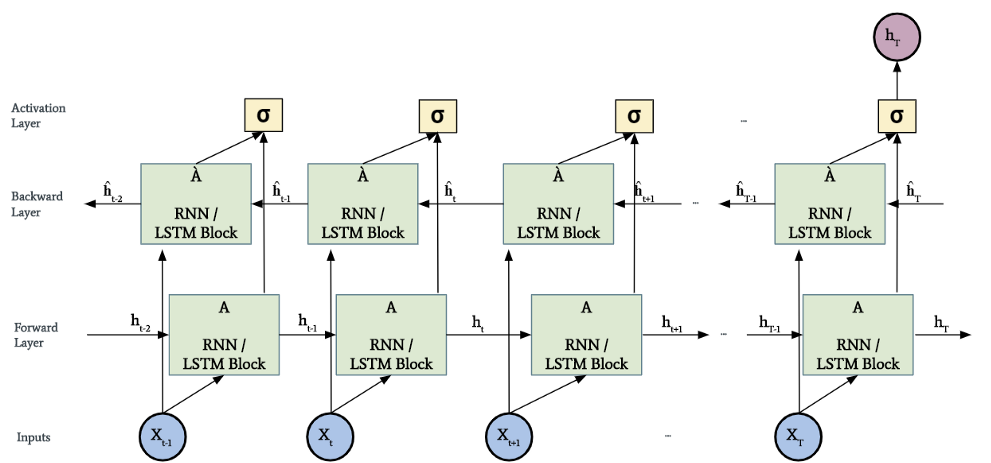
\includegraphics[width=\textwidth]{images/b-lstm}
    \caption{Example Bi-directional long short-term memory neural network with an output state per input and a single output after all inputs are processed.}
    \label{fig:b-lstm}
\end{figure}
As mentioned earlier, SRNN and FRNN suffer from very very good short-term memory while lacking long-term memory. To account for this Long Short-Term memory units were introduced \cite{Hochreiter1997long}. These units were meant to replace the `normal' neurons in a FRNN. LSTM units are different from normal neurons by its inner structure. Normal RNN units work like neurons in a multi-layer perceptron, however instead of only adding up all inputs (or outputs from previous layer), previous outputs are also added to this sum.

A LSTM unit contains an internal state which acts as its memory. An input, output and forget gate decide how the internal state is changed. The way these are set up enables a LSTM to `remember' important data and `forget' less important data of all the data or current input. \textcite{Li2015constructing} found these properties especially suitable for Speech Recognition (`forget' noise, `remember' phonemes), while \textcite{Sak2014long} used these properties for acoustic modeling, because of its performance on time sequence data.

A LSTM network can receives a series of input. The network can then return one output per input sample (sequence-output) or return one output once all inputs are processed (single-output). If one is interested in predicting the word someone is typing, sequence-output can be used. If only the next word needs to be predicted after someone is done typing the previous word, single-output can be used.

A bi-directional (recurrent) neural network, first introduced by \textcite{Schuster1997bidirectional}, is a special kind of recurrent neural networks. A B-RNN works by not only using the input data up to a certain frame, but also the input data from the end to that certain frame. Training thus is performed in both positive and negative time direction. Using both time directions during training enlarges the context of a recurrent unit and was therefore proven to increase the performance of a model. An example of a single-output bi-directional LSTM network can be found in \autoref{fig:b-lstm}.\\

Going back to \citeauthor{Gimeno2020a}; by using a bi-directional RNN with LSTM units, they reported a relative improvement of 19.72\% and 5.35\% compared to the best results in the literature at that moment for their two datasets (Albayzín 2010 and 2012) respectively. 

\subsubsection{Applications of AAS models}
Many applications of models capable of performing such segmentation and classifications are within the broadcast data domain. For example in a live radio broadcast these models can be used to automatically apply the right type of audio filtering onto the broadcast audio stream. This could be an audio filter focused on higher tones when someone is talking or an audio filter focused on lower tones when music is played. Also automatically distinguishing when a person's voice is transmitted through a microphone or background noise, can be used to automatically cut the audio feed of a microphone during a live broadcast.

Non-real time applications of these models are within audio indexing and retrieval of for example documentaries, podcasts or other broadcasts. Audio streams automatically segmented by these models can then be used to speed up the process of retrieving certain parts from documentaries or cut all parts where nobody is talking in a podcast.

By modifying these existing models and extending them from multi-class \textbf{audio} segmentation to multi-class \textbf{music} segmentation will also benefit this field by giving it more specific classes within the music class. Although these models aim to find different kind of patterns within the features used\footnote{I will elaborate on this in the \nameref{sec:acoustic_features} section below.}, the basic principles can be used to decrease the effort needed to create a good performing music segmentation model that uses machine learning.


\section[CNN in MIR]{Convolutional Neural Networks in Music Information Retrieval}
\label{sec:cnn_related}
Another type of machine learning commonly used in another field of computer science and adapted to be useable in \mir\ are Convolutional Neural Networks (CNN). CNN's, first introduced by \textcite{Lecun1989backpropagation} for recognizing handwritten postal codes, and later most improved by \textcite{Krizhevsky2012imagenet}, is a type of artificial neural network that are specialized for processing --most often classifying-- data that has a known grid-like topology. This, as were its first applications, generally is image data, because images have a very well-defined grid-like topology. While binary images being the most simple form of two-dimensional images with for each pixel only 2 possible values, more complex images, like multi-channel images (red-green-blue images, cyan-magenta-yellow-black images) or multi-view images (top view, bottom view, etc,) can be processed too, albeit in a slightly different way.

Convolutional networks are inspired by the neural architecture found in the human visual cortex by \textcite{Hubel1968receptive} in the V1 and V2 area \cite{Lindsay2020convolutional}. Each neuron in the V1 area is sensitive to a sub-region of the visual field, called a \textit{receptive field}. The activation of each neuron then depends on the occurrence of certain visual features (like edges in certain orientations) in the receptive field. The receptive fields are tiled to cover the entire visual field. The current way to imitate this receptive field is to use convolutions, hence the name of this type of artificial neural network. A convolution, or kernel, is a filter that is applied on an image. This way, each neuron in the next layer is connected to a sub-region in the output or image of the layer before (\autoref{fig:cnn_example}). During training, neurons of deeper convolutional layers learn to adapt their weights in such a way that the neuron activates on certain patterns found in the (convolved) image from the layer above, similar to how the neurons in the different visual areas in the visual cortex work.

Feature vectors at first don't seem to be multi-dimensional 'images' however when put in a time sequence one can construct a two-dimensional matrix from multiple one-dimensional feature vectors. This principle makes it possible to also apply convolutional neural networks to natural language processing (NLP) \cite{Lopez2017deep} and music information retrieval. In the case of NLP, each word in a sentence is first converted to a feature vector by either embedding it \cite{Ghannay2016word,Mikolov2013efficient}, or using one hot encoding. The feature vectors of multiple words concatenated then can be used as two-dimensional input for a CNN, slightly imitating the way N-grams work \cite{Brown1992class}.

\textcite{Basili2004classification} were the first to apply machine learning on automatic genre classification of songs. However, they only used Naïve-Bayes, Voting Feature Intervals, Decision Trees and Nearest-Neighbors classifiers. \textcite{Li2010automatic} actually were the first to use convolutional neural networks for automatic genre classification. They were therefore the first to use convolutional neural networks in music information retrieval, and make use of the one-dimensional feature vector concatenation into two-dimensional 'images'. Although they reach over 85\% accuracy when using a dataset with only 3 genres, their accuracy heavily decreases to under 30\% when they use a dataset with 6 genres.
\begin{figure}[t]
    \centering
    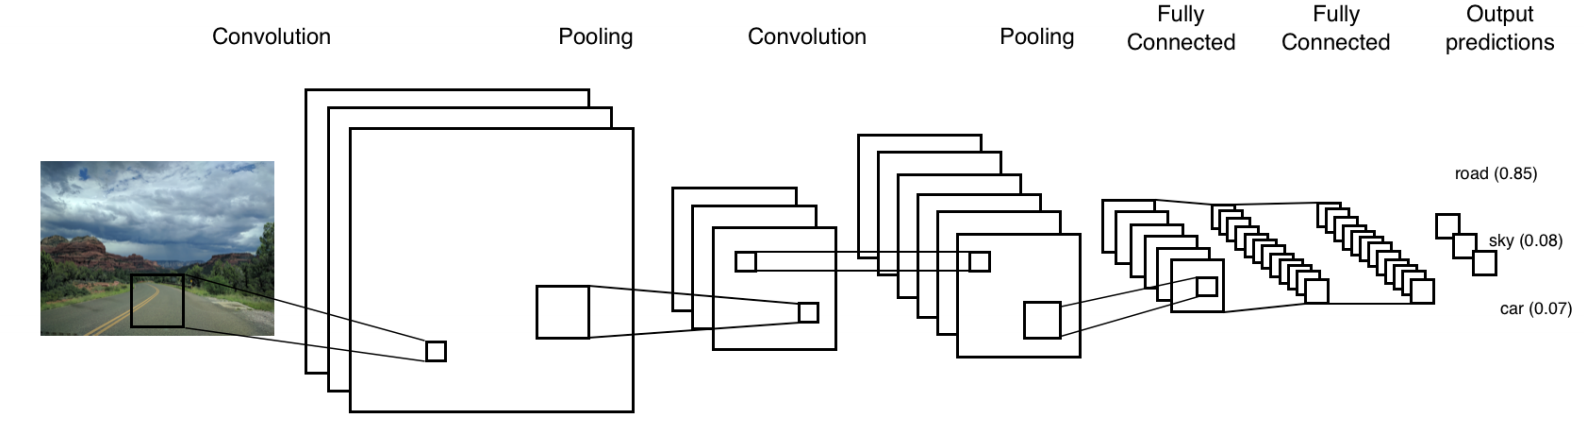
\includegraphics[width=1\textwidth]{images/cnn_example}
    \caption{Basic structure of a convolutional neural network.}
    \label{fig:cnn_example}
\end{figure}

\subsection[CNN for onset detection]{Convolutional Neural Networks for onset detection}
\begin{figure}[t]
    \centering
    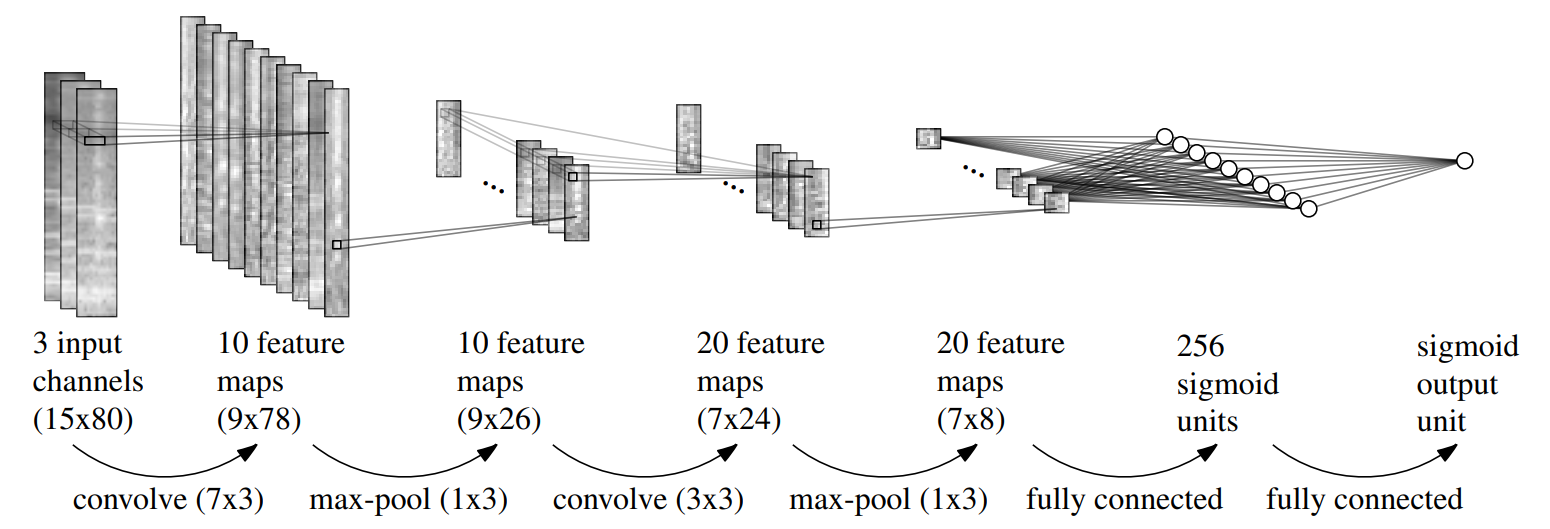
\includegraphics[width=1\textwidth]{images/onset_detection_cnn}
    \caption{Final CNN created for onset detection, starting from a stack of three spectrogram excerpts, ending with one output unit indicating the chance of an onset.\\
    Reprinted from \textcite{Schluter2014improved} (Figure 2).}
    \label{fig:onset_detection_cnn}
\end{figure}
The next subdomain of MIR --related to MSA-- where convolutional neural networks are used with great success, is within musical onset detection.

Musical Onset Detection is the process of automatically extracting the point of time of the musical onsets within a piece of music. A (musical) onset is the beginning of a musical event, most often the beginning of a musical note, but may also be other musical events \cite{Bello2005tutorial,Zhou2011music}. It was first introduced as a contest by Paul Brossier and Pierre Leveau for the MIREX 2005 \footnote{\href{https://www.music-ir.org/mirex/wiki/2005:Audio_Onset_Detect}{See the MIREX website for their proposal. (link)}}. From this moment it has been an annually recurring contest of the MIREX.

Again, using machine learning was on equal performance or outperformed state-of-the-art at that time \cite{Eyben2010universal}. However, in contrast to the current models at that time, this new approach was able to perform real time onset detection by actually predicting the onsets. The proposed model, in multiple ways improved by \citeauthor{Bock2012online}, using a recurrent neural network with long short-term memory (LSTM) units produced a 0.840 F-measure on real time onset detection compared to 0.826 and 0.866 F-measure on non-real time onset detection by state-of-the-art models at that time \cite{Bock2012online}.

After this success with the application of recurrent neural networks for onset detection, \textcite{Schluter2013musical} propose an onset detection method using a convolutional neural network. Not only did this model perform better than the (improved) bi-directional recurrent neural networks at that time (0.885 F-measure compared to 0.873), it also required less (manual) pre-processing, since CNN's are able to 'learn' this pre-processing in their first layer(s). A year later \textcite{Schluter2014improved} report improvements made on the initially proposed model, bringing its F-measure above 0.9 to 0.903 respectively (\autoref{fig:onset_detection_cnn}). \citeauthor{Schluter2014improved} explain the high performance of CNN's on onset detection by their accuracy in finding oriented edges in images. Musical onsets show up as 'edges' in spectrograms of a piece music and a CNN is therefore perfectly suited for finding these edges and thus the onsets\footnote{In practice this is a lot less trivial, however \textcite{Schluter2014improved} have put great effort into trying to explain it.}.

After these successes with the application of CNN's within musical onset detection, \citeauthor{Ullrich2014boundary} made the link to musical structure analysis and its similarity to musical onset detection. Their efforts to also apply convolutional neural networks on this music information retrieval problem resulted in a new state-of-the-art for music structure analysis, which I will describe below.


\section[MSA]{\msa}
Music Structure Analysis, as described in the introduction, is the process of finding important parts in a piece of music, on many possible hierarchical levels. As per my definition I will focus on the functional high level segments in a piece of music. 

In many songs, a few of these high level segments have the same function, and are therefore grouped together. This thus resulted in the two approaches to this problem described in the introduction. Due to the many differences between different songs, even within the same genre, it has always been very difficult to assign a function to a segment. First research to this problem therefore initially focused on finding the segment boundaries first and then group similar segments together. Similar segments were then given the same capital letter denoting their similar function without specifying it further (as verse, chorus, etc.).

\subsection[DSA approach to MSA]{\dsa\ approach to \msa}
\begin{quote}
    \textbf{N.B.} A more in depth overview of the \dsa\ approach can be found in \textcite{Jesperthesis}.
\end{quote}
The DSA approach can be summarized into a few different sub-approaches; a novelty-, homogeneity- and repetition-based approach.

\subsubsection{Self-Similarity Matrix}
\begin{figure}[t]
    \centering
    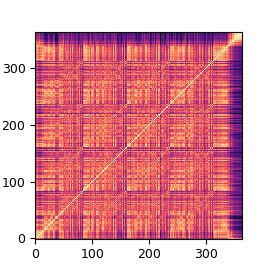
\includegraphics[width=.5\textwidth]{images/ssm}
    \caption{Example of a Self-Similarity Matrix, created on \textit{Mrs. Robinson} by Simon \& Garfunkel.\\
    Reprinted from \textcite{Jesperthesis} (Figure 2.2a).}
    \label{fig:ssm}
\end{figure}
All methods rely on the same main principle, a self-similarity matrix (SSM). A self-similarity matrix, first introduced by \textcite{Foote1999visualizing}, is a matrix calculated by calculating the distance of each feature vector to the other feature vectors. Lower distance values mean that the two feature vectors compared are more similar to each other than two feature vectors with a higher distance value. This will result in a $n\times n$ matrix, where $n$ is the amount of feature vectors of the song. The distances are then normalized to a similarity value. If the distance between two feature vectors is equal to 0, their similarity is equal to 1, all other distance are normalized between a similarity value of 0 and 1. From the way self-similarity matrices are calculated, a diagonal line of similarities with a value of 1 will be seen. This line represents the similarity between each feature vector and itself, which is obviously 1.

\subsubsection{Repetition-based Approach}
The repetition based approach to DSA makes use of this property of SSM's by detecting more diagonal lines in the SSM. Another diagonal line means that a certain part of the song is repeated elsewhere. The start and end of these repetitions can than be used to determine the location of a segment boundary. One technique used to do this is called \textit{Structure Features} \cite{Serra2012unsupervised}. A (cyclic) time lag matrix is constructed from a SSM. This time lag matrix shows horizontal or vertical lines (depending on the exact process used), a line shows for the frame the line occurs in, the amount of time (in frames) it takes before that frame is repeated (in terms of the feature used to create the time lag matrix).

\subsubsection{Novelty-based Approach}
\begin{figure}[t]
    \centering
    \begin{subfigure}{.5\textwidth}
        \centering
        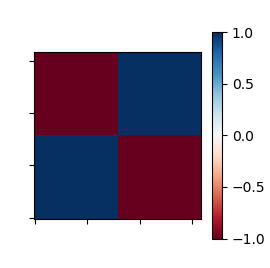
\includegraphics{images/checkerboard}
        \caption{Normal checkerboard kernel}
        \label{pw:fig:foote:norm}
    \end{subfigure}%
    \begin{subfigure}{.5\textwidth}
        \centering
        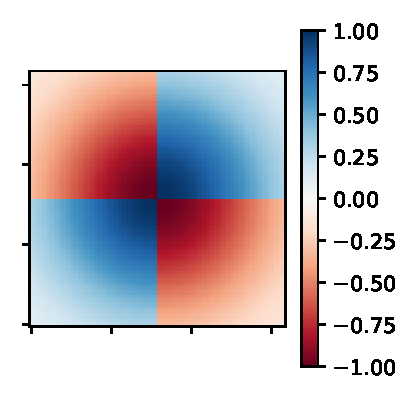
\includegraphics{images/gaussian_checkerboard}
        \caption{Gaussian tapered checkerboard kernel}
        \label{pw:fig:foote:gaus}
    \end{subfigure}
    \caption{An example of a normal and Gaussian tapered checkerboard kernel.\\
    Reprinted from \textcite{Jesperthesis} (Figure 2.3).}
    \label{fig:checkerboard}
\end{figure}
The novelty based approach makes use of another property of SSM's: blocks. A block in a SSM denotes a section of consistent features for the duration of the block. \textcite{Foote2000automatic} was the first to come up with a way to detect the transition of one block into another along the main diagonal of the SSM. Their method used a (Gaussian) checkerboard kernel. A most basic checkerboard kernel can be constructed using a $2\times2$ matrix, like this:
$$\mathbf{K} = \begin{bmatrix} -1 & 1 \\ 1 & -1 \end{bmatrix}$$
It functions similar to how a \textit{Sobel Operator} works in image processing to detect edges. However, where the \textit{Sobel Operator} uses a horizontal and vertical operator to detect horizontal and vertical edges, a checkerboard kernel is specifically designed to detect diagonal edges.

Since this is a $2\times2$ matrix, only 2 different feature vectors will be taken into account, it is therefore more common in music structure analysis to use larger checkerboard kernels, like $64\times64$. To give more importance to closer feature vectors, the checkerboard matrix can be tapered with a Gaussian function (\autoref{fig:checkerboard}).

By applying a checkerboard kernel over the diagonal of a SSM, an 'edge activation' can be calculated for each feature vector. From this a \textit{novelty curve} can be constructed, denoting the amount of novelty (in terms of the acoustic features used) between two adjacent feature vectors. By, for example, applying adaptive thresholding, the peaks in this novelty curve can be extracted. The location of each peak then stands for the location of a segment boundary.

\subsubsection{Homogeneity-based Approach}
The homogeneity-based approach to DSA has been researched a lot less. A most recent research implements this approach using a Hidden Markov Model. Each state stands for a homogeneous piece of music, and the chance to go to the next state determines the chance of a segment boundary.

\subsubsection{2D fourier Magnitude Coefficients}
Once all segment boundaries are detected, the segments can be extracted. Then all segments need to be labeled. One of the most common ways is to use some kind of clustering method, and then assigning a label to each cluster. Each segment, however, can be of different length. A way to represent each segment in such a way that a distance metric could be applied was therefore needed. The use of the magnitude of the 2D Fourier Transform, originally a technique used in image processing, was therefore first introduced by \textcite{Ellis2007beat}. \textcite{Nieto2014music} were the first to apply the 2D Fourier Magnitude Coefficients for segment clustering.

Clustering segments this way proved to be quite accurate. One big problem however, was the amount of clusters that had to be used, since this could vary per song.

\subsection{Current State-of-the-Art}
\begin{figure}[t]
    \centering
    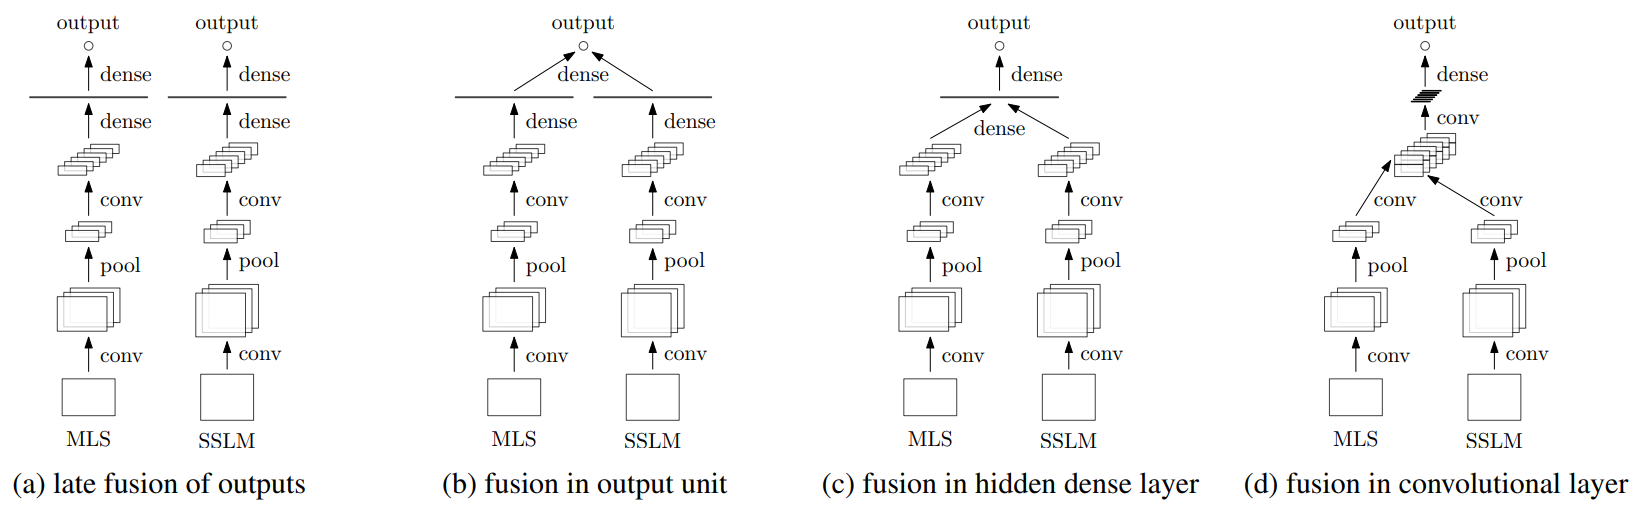
\includegraphics[width=1\textwidth]{images/fusion_examples_cnn}
    \caption{Four different CNN architectures for combining two input features.\\
    Reprinted from \textcite{Grill2015music}.}
    \label{fig:fusion_examples_cnn}
\end{figure}
Due to the successes of CNN's within onset detection and its similarity to finding the segment boundaries --the start of a new high level segment can be compared to a strong onset viewed in a big time window-- , \citeauthor{Ullrich2014boundary} therefore put their effort into creating a convolutional network that is capable of finding these boundaries, based on their model created for onset detection. They presented their first results in \citeyear{Ullrich2014boundary} \cite{Ullrich2014boundary}. They report an advance of state-of-the-art of that time for MSA, F-measure of 0.33 to 0.46 for 0.5s tolerance and F-measure of 0.52 to 0.62 for 3s tolerance.\footnote{A 0.5 or 3 second tolerance means that a segment boundary is counted as a hit if it lies within 0.5 or 3 seconds of the ground truth. Refer to \textcite{Jesperthesis} (section 2.2.2) for more elaboration on this subject.} A few different input features were tested (MFCC, Chroma, Mel spectrograms), and finally 5 different models trained on Mel spectrograms were bagged \cite{Breiman1996bagging} together for their final model.

To account for misses of boundaries between non-local musical cues, such as segment repetitions, \textcite{Grill2015music} present an improvement on the initial convolutional network by combining the Mel-scaled Log-magnitude Spectrograms (MLS) with Self-Similarity Lag Matrices (SSLM) as input. They test different models that each combine these inputs at a different moment in the model (\autoref{fig:fusion_examples_cnn}). Their best model, fusing the inputs in the convolutional layer (\autoref{fig:fusion_examples_cnn}d), advanced the F-measure from 0.46 \cite{Ullrich2014boundary} to 0.52.

\textcite{Grill2015music2} further expanded this model by dividing the SSLM into a near (14 second time context) and far (88 second time context) variant, each used as different feature combined with a MLS as their input for their models. They also added another neuron to the output layer giving it two neurons in total. One of these neurons was trained on lower level annotation available in their dataset, while the other neuron was trained on the high level annotation. They show that using two annotation levels increases the F-measure of over 0.3 on 0.5s tolerance.

They present their final model in their MIREX submission for the MIREX 2015 Music Structural Segmentation task \cite{Grill2015structural}.


\section{SALAMI Dataset}
\label{sec:salami}
Many datasets have been created and used for music structure analysis. An extensive listing with most well-known data-sets can be found on \href{https://ismir.net/resources/datasets/}{the website of the International Society of Music Information Retrieval (ISMIR)}. There are a total of 16 data-sets listed there that cover musical structure. Only 5 of these data-sets cover western popular music and feature a song total above 100, these are the INRIA:Eurovision, INRIA:Quaero, QMUL:Beatles, RWC and SALAMI datasets respectively.\\
Although these datasets contain the annotations, and some of them also the features, of the songs, none of these actually provide the audio of the annotated songs.\\
The only dataset that did provide a link to the audio files is the SALAMI dataset. The SALAMI dataset, or \textit{Structural Analysis of Large Amounts of Musical Information} dataset, is an unprecedented large dataset that contains 2400 structural annotations \cite{Salami}. This dataset contains, among many other subsets, an \textit{internet archives} subset. The internet archives subset contains the annotations of songs publicly available on the internet together with a link to an mp3 file with the audio.


\section{Acoustic Features}
\label{sec:acoustic_features}
To represent the audio in a more meaningful way, many features have been used or proposed in the past, in this section I will inspect a few of most popular features that are being used or have been used in music information retrieval and music structure analysis in particular. Further explanation of these features among citations to great other sources about these features can be found in \cite{Paulus2008acoustic}.

\subsection{Chroma}
\begin{figure}[t]
    \centering
    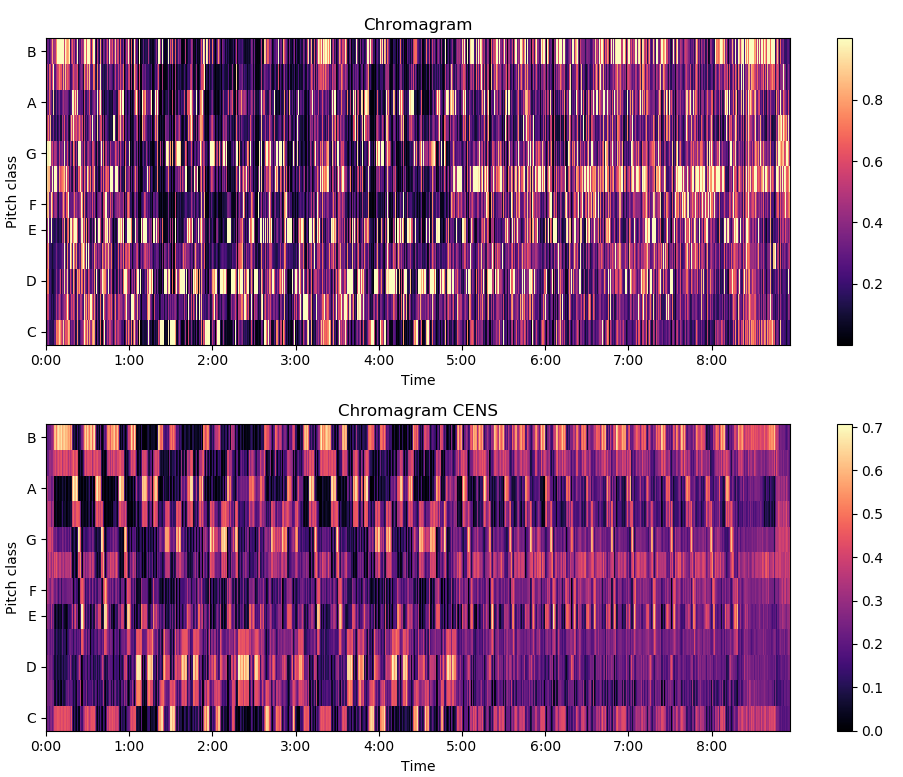
\includegraphics[width=\textwidth]{images/cqt_cens}
    \caption{PCP chromagram compared to CENS chromagram, both constructed with 12 bins, 2048 FFT window size and 512 hop length.}
    \label{fig:pcp_cens}
\end{figure}
The chroma, or 'color', of a song closely relates to the (often twelve) different pitch classes in music. There are multiple chroma types, each one calculated in a different way to represent each pitch class in a slightly different way. The first step for each chroma type however, is to first create a \textit{spectrogram}. A spectrogram is created by applying the discrete fourier transform (DFT) on a slice, or \textit{window}, of the audio. By repeatedly applying the DFT on the window, while it is being slid or hopped through the audio, one can create a representation of the intensity of each frequency over time. This technique is called the \textit{Short Time Fourier Transform} (STFT). 

The window size in this context is called the Fast Fourier Transform or \textbf{FFT window size} (often 2048 or 4096 audio samples). Each time the window is moved, the amount of audio samples it moves is called the \textbf{hop length} (often 512 or 1024). If a FFT window size of 4096 is used and a hop length of 1024, one can see that there is 75\% overlap between each output of the DFT.

The \textit{Pitch Class Profile} (PCP) \cite{Lee2006automatic} is one of the most low-level chroma representations. The STFT spectrogram is converted to an intensity of each 12 pitch classes ($C$, $C\sharp$, $D$, etc.) on the equal-tempered scale. If 12 bins are used, each bin represents a semitone, if a multiple of 12 bins are used, each bin represents an equal fraction of a semitone. The PCP has primarily been used to compute the similarity between two songs, however more computation and analysis is needed to extract higher-level patterns from the PCP.

The \textit{Chroma Energy Normalized Statistics}, or CENS, chroma representation \cite{Muller2005chroma} is another chroma representation commonly used in audio matching, audio retrieval and music similarity. This feature is more popular in this fields because of its robustness to audio dynamics, timbre and articulation. This robustness is obtained by taking statistics over large windows, therefore smoothing local deviations in tempo, articulation and music ornaments such as trills and arpeggiated chords. A downside to this smoothing is that at some points in time it can be hard to determine which pitch class is the most dominant.

A comparison between a PCP chromagram and CENS chromagram can be found in \autoref{fig:pcp_cens}.

\subsection{Timbre}
\begin{figure}[t]
    \centering
    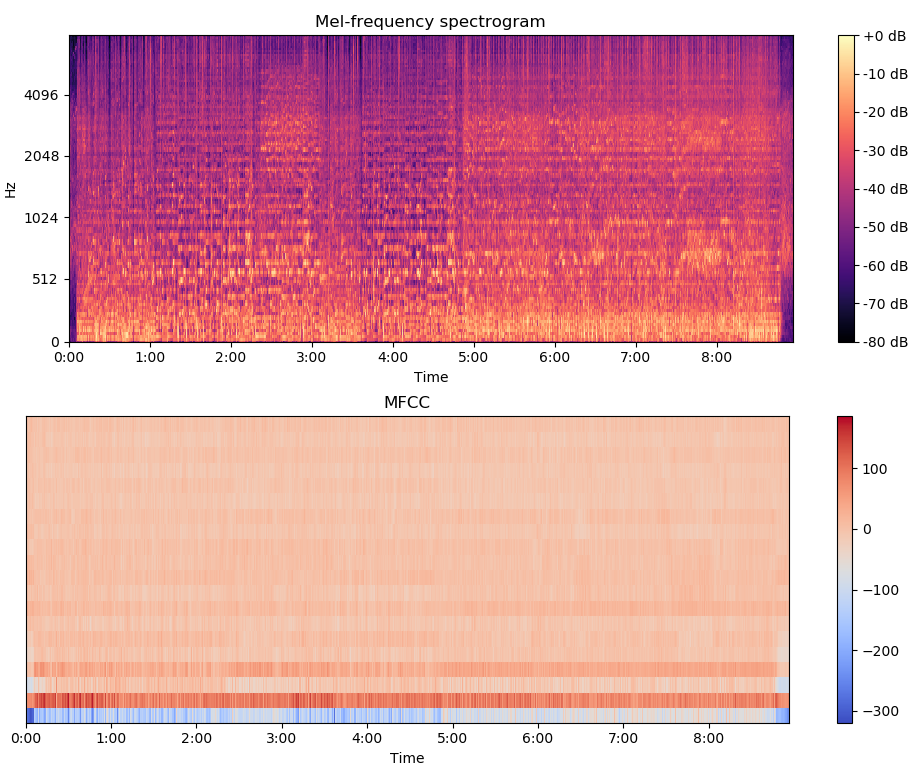
\includegraphics[width=\textwidth]{images/mls_mfcc}
    \caption{Mel-frequency spectrogram compared to Mel Frequency Cepstral Coefficients with 20 bins.}
    \label{fig:mls_mfcc}
\end{figure}
Another way of representing audio is by its timbre. Timbre has no direct definition, it however is generally described as \textit{'The perceived sound quality of a musical note, sound or tone'}. Timbre was introduced to distinguish between two instruments, since two instruments playing the same tone, will have the same chroma value.

While the Fourier Transform is able to extract the intensity of each frequency, it has a few flaws. That is why the Mel Scale was created. The mel scale, originally introduced by \textcite{Stevens1937scale}, is a perceptual scale that scales each pitch judged by listeners to be in equal distance from each other. They introduced this scale because the human auditory system is not equally sensitive to each audio frequency, for example the human auditory system is most sensitive to the 2000 to 5000 Hz range \cite{Gelfand1997essentials}, while the screams of a baby are around the 3500 Hz region. 

Using the mel scale we can create so-called Mel-scaled spectrograms, or cepstrograms, that represent the intensity of each mel-frequency at each audio sample. A cepstrogram does represent the different sounds quite good, especially since the vector length at each time point is a lot longer than 12 (or a low factor of thereof). However, due to its enormous dimensions, using a cepstrogram as feature for a model can be quite computational intensive.

Partly for this reason, the \textit{Mel Frequency Cepstral Coefficients} (MFCC) were created \cite{Logan2000mel}. The MFCC discretize a mel-scaled spectrogram by first taking the Fourier Transform of an audio stream. Then, the powers of the spectrum is mapped onto the mel-scale, using triangular overlapping windows. The log of the power of each mel frequency is taken, followed by a discrete cosine transform over the list of mel log powers. Often 20 bins are used for the final vector length of the MFCC. A comparison between a mel-scaled spectrogram and the MFCC of that same spectrogram can be found in \autoref{fig:mls_mfcc}.

Although its high information density, MFCCs are not 'the ultimate feature to describe all audio' \cite{Pachet2004improving}. Therefore, other timbre features still need to be considered, one example being the \textit{Constant-Q Transform} (CQT) \cite{Brown1991calculation}. The CQT is very closely related, but is calculated in a slightly other way. However, due to the complex calculation, another way of calculating the CQT using the FFT in conjunction with a kernel was proposed \cite{Brown1992efficient,Blankertz2001constant}.

\subsubsection{Rythm}
\begin{figure}[t]
    \centering
    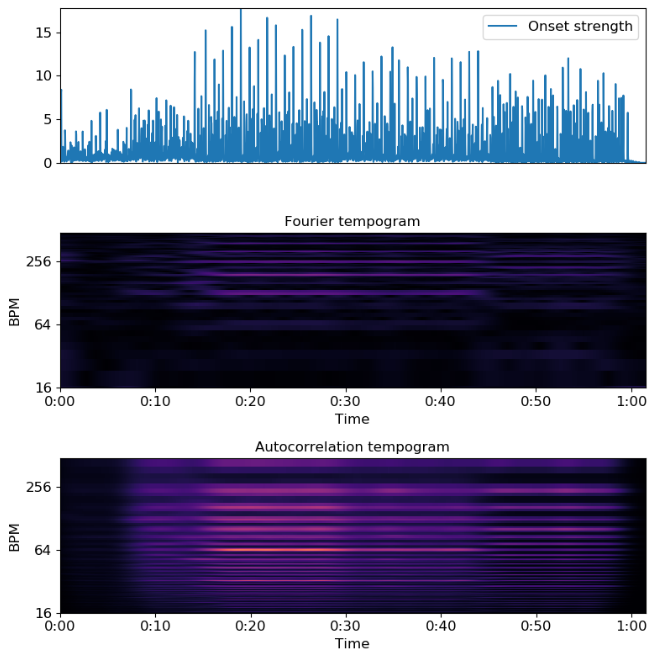
\includegraphics[width=\textwidth]{images/tempogrammi}
    \caption{A comparison of a Fourier tempogram and autocorrelation (cyclic) tempogram made on the same onset strength envelope.}
    \label{fig:tempogrammi}
\end{figure}
Not only the tones or harmony of a piece of music can be used as input for music information retrieval models, rhythmic features can also add a lot of information. This is especially applicable to the detection of the musical structure. Similar segments often employ similar rhythmic features, while different segments, like verse and chorus, can differ a in their rhythmic. Rhythmic features therefore can be used to both label or cluster segments. or to detect boundaries between two segments (when a sudden change in a rhythmic feature is detected).

One of the most well known rhythmic features will be tempo. Tempo can be represented as the amount of beats per minute (BPM). Tempo represented on a time scale is called a \textit{tempogram}; the feature vector at each time point represents the probabilities of a certain BPM at that time point. 

Since detecting the tempo at each time point turned out to be quite difficult, cyclic tempograms were introduced \cite{Grosche2010cyclic}. A cyclic, or autocorrelation, tempogram detects tempi differing with a power of two, thereby reducing the amount of possible tempi at a certain time point, and thus increasing the probability value of the most probable tempo, since there will be more tempi differing with a power of two around the true tempo.

Another way of computing a tempogram is by using a (short-time) Fourier transform on the onset strength envelope. A comparison between these tempograms can be found in \autoref{fig:tempogrammi}.

\chapter{Methodology}
\label{ch:method}
This chapter contains an extensive explanation of the dataset and the labels and acoustic features that were extracted from it. I then introduce the architectures of the models I have created.


\section{The Data}
\label{sec:3.the_data}
As explained in the \nameref{sec:salami} section, I will be using the internet archives subset of the SALAMI dataset as data for the models I will create. Another benefit of using this dataset, apart from the amount of publicly available songs, is that the SALAMI dataset, and the internet archives subset in particular, have been part of the evaluation datasets for many MIREX Music Structural Segmentation contests. The results produced by the models I will create will therefore be quite comparable to the results reported in the many MIREX submissions to this specific MIREX contest.

The internet archives subset consists of two parts: A CSV file containing all metadata about each song and the actual annotations. Among this metadata is a web-link to the audio file of that song in mp3 format. Using these links and the SONG ID given to each song, each audio file was downloaded and saved as \textit{[song-id].mp3}.

All annotations for a song are stored in a folder named by the ID of the song. Since one or two annotators have annotated each song, this folder may contain one or two text files. Each line of text in these text files stand for a segment; the first number denote the time point (in seconds) of the start of the segment. Then the labels describing the function of the segment follow. Because two levels of annotation were used, the collection of labels may contain one or more items.

The first item in the collection of labels always is a lowercase letter describing the low level function of the segment, often written in combination with a \textit{'}. Segments with the same label are musically similar to each other, the \textit{'} means that although the (musical) function between the segments is similar, they differ slightly in musical terms (e.g. key, mode).

Some collections of labels contain two more labels, the high-level annotation (denoted by an uppercase letter) and the segment function (chorus, verse, etc.). All time points without high-level annotation and segment function implicitly have the most recent high-level annotation and segment function that occurred. 

Apart from the text files containing all annotations of one annotator, the folder with annotations also includes a folder for each annotator. In this folder there are multiple text files each one containing one type of annotation, thus one text file contains the low-level annotations, another one contains the segment functions, etc.

The exact instructions given to each annotator on how to annotate a song, and how to format their annotations can be found in the \href{https://github.com/DDMAL/salami-data-public/blob/master/SALAMI%20Annotator%20Guide.pdf}{annotator's guide (link)}.

Using the time points and labels of each segment boundary I will be able to evaluate the accuracy of each model to predict the start of each segment within a 0.5 second and 3 seconds tolerance, I will further explain the exact evaluation method in the \nameref{sec:eval_meth} section. The full list of songs used can be found in \autoref{app:dataset}.

\subsubsection{Label extraction}
\begin{table}[t]
    \centering
    \begin{tabular}{|l|l|l|l|}
    \hline
    \textbf{Label}         & \textbf{Occurrence in data} & \textbf{Grouped Label} & \textbf{Occurrence in data} \\ \hline\hline
    silence       & 446                & \textbf{silence}       & 446                \\ \hline
    no\_function  & 483                & \textbf{no\_function}  & 505                \\ \hline
    applause      & 12                 & no\_function  &                    \\ \hline
    stage\_sounds & 6                  & no\_function  &                    \\ \hline
    spoken        & 3                  & no\_function  &                    \\ \hline
    crowd\_sounds & 1                  & no\_function  &                    \\ \hline
    intro         & 243                & \textbf{intro}         & 300                \\ \hline
    head          & 57                 & intro         &                    \\ \hline
    verse         & 718                & \textbf{verse}         & 726                \\ \hline
    pre-verse     & 7                  & verse         &                    \\ \hline
    voice         & 1                  & verse         &                    \\ \hline
    interlude     & 189                & \textbf{interlude}     & 249                \\ \hline
    transition    & 51                 & interlude     &                    \\ \hline
    break         & 9                  & interlude     &                    \\ \hline
    solo          & 514                & \textbf{solo}          & 717                \\ \hline
    instrumental  & 160                & solo          &                    \\ \hline
    theme         & 39                 & solo          &                    \\ \hline
    main theme    & 4                  & solo          &                    \\ \hline
    chorus        & 655                & \textbf{chorus}        & 740                \\ \hline
    pre-chorus    & 61                 & chorus        &                    \\ \hline
    post-chorus   & 24                 & chorus        &                    \\ \hline
    bridge        & 106                & \textbf{bridge}        & 107                \\ \hline
    build         & 1                  & bridge        &                    \\ \hline
    outro         & 132                & \textbf{outro}         & 182                \\ \hline
    coda          & 48                 & outro         &                    \\ \hline
    fade-out      & 2                  & outro         &                    \\ \hline
    \end{tabular}
    \caption{Grouping of all 26 unique labels into 9 main labels.}
    \label{tab:label_grouping}
\end{table}
To not have to manually parse each text file I have made use of the formatted annotations in Json Annotated Music Specification (JAMS) format \cite{Humphrey2014jams}. These formatted annotations are available in the Music Structure Analysis Framework (MSAF) \cite{Nieto2016systematic}.

For each song in the internet archives dataset I've chosen the first annotation. This reduced the amount of different annotators to under 5, thereby decreasing the amount of ambiguity between the annotations of different songs. Still, there were quite a lot of different labels present in the dataset (26), of which 10 labels have around or under 10 occurrence within the 4000 segments present in the first annotation of each song in the internet archives dataset.

By decreasing the amount of unique labels, I further decreased the amount of ambiguity between the annotations and presumably increased the accuracy of the models. I've based the grouping on occurrence of the unique label in the dataset, its musical function and the label of another annotator for the same segment. By also listening to a few segments of each of the labels that had a low occurrence in the data, I could also use my own judgement of the relation between a certain label and its associated sounds for the grouping of the labels. 

One example are the segments that were labeled as \textit{instrumental}. These segments turned out to be musically equal to \textit{solo} in the context of the data. Since the data primarily consists of live recordings of (alternative) Western Popular Music, both meant a sole guitar (supported by drums) without any lyric. I therefore chose to group these labels together as \textit{solo}. For the other label groupings a similar process was performed as well, while the other factors described were taken into account as well. The final grouping of each label can be found in \autoref{tab:label_grouping}.

Once each raw label was converted to its grouped label, a one-hot-encoding vector of each label was created. A one-hot-encoding vector of a beat is a vector with the length of the amount of labels containing only zeros except for the index of the true label for that beat. The indices of the grouped labels are 0 to 8 for \textit{silence, no\_function, intro, verse, interlude, solo, chorus, bridge} and \textit{outro} in that specific order respectively.


\section{Feature Selection}
\subsubsection{Feature Extraction}
\begin{table}[t]
    \centering
    \begin{tabular}{|l|c|c|}
    \hline
    \textbf{Feature} & \textbf{Vector Length} & \textbf{Matrix Size}  \\ \hline\hline
    CQT       & 84          & $84\times4$  \\ \hline
    CENS      & 12          & $12\times4$  \\ \hline
    PCP       & 12          & $12\times4$  \\ \hline
    Tonnetz   & 6           & $6\times4$   \\ \hline
    MFCC      & 14          & $14\times4$  \\ \hline
    Tempogram & 192         & $192\times4$ \\ \hline
    \end{tabular}
    \caption{Vector length and matrix size of each feature extracted.}
    \label{tab:feature_sizes}
\end{table}
I used the LibROSA Python package for music and audio analysis \cite{Mcfee2015librosa} to extract the features from each audio file. I have used a hop length of 1024 together with a FFT window of 4096 for 75\% overlap within each feature vector.

First the beats were extracted using the method introduced by \textcite{Ellis2007beat}.
Then the Chroma Energy Normalized Statistics (CENS) \cite{Muller2005chroma} chroma variant was extracted. As low level harmonic/chroma features I extracted the Pitch Class Profile (PCP) \cite{Lee2006automatic}. I saved the PCP as self-contained feature and used it to create the Tonnetz features \cite{Harte2006detecting}. I also created a Mel Spectrogram \cite{Stevens1937scale} and used it to create the Mel-Frequency Cepstral Coefficients (MFCC) with 14 coefficients \cite{Logan2000mel}, these represent the timbre of the song. As other timbre feature I extracted the Constant-Q Transform (CQT) \cite{Brown1991calculation}, using the technique described by \textcite{Schorkhuber2010constant}. Because often a segment boundary goes hand in hand with a change in tempo (e.g. a short speedup in tempo, or the next segment is in a lower or higher tempo), I extracted the tempogram of each song with a window length of 192 \cite{Grosche2010cyclic}. 

The resulting feature vectors have a length of 84, 12, 12, 6, 14 and 192 for the CQT, CENS, PCP, Tonnetz, MFCC and tempogram feature vectors respectively (\autoref{tab:feature_sizes}).

\subsubsection{Data Reduction}
Each feature was first extracted based on the frames of a song. The amount of frames of a song is calculated by the sample rate (amount of audio samples per second) multiplied by the length of the song (in seconds) divided by the hop length. Each song is converted to Waveform (wav) audio format with a sample rate of 22050, this combined with a mean song length of 4 minutes or 240 seconds and a hop length of 1024 for each feature results in $(240\cdot22050)/1024=5168$ frames on average for each song. 

To reduce the amount of feature vectors I have beat synced each feature. The means that for each beat in a song there is one vector for each feature. This vector is calculated as the average of all vectors of that feature within the beat. With an average beats per minute (BPM) of 120 for all songs (thus 2 'frames' per second), the average amount of vectors per song is now reduced to $240\cdot2=480$. With a total of 377 songs (after data cleaning) I gathered a total of about 180000 vectors per feature.


\section{Proposed Architectures}
\subsection{Preserving Temporal Aspect of Music}
To obtain faster learning speeds of the models, the data needs to be shuffled; if all beats of a song are kept in the initial order, the output labels will be sequences of the same label. Even when the batch size is increased, samples with the same output label are still being fed to the network in each learning iteration, thus lowering its capabilities to learn multiple output labels in one learning iteration.

One problem of shuffling the data however is that one beat alone will not be enough for a network to learn all patterns that can be associated with an output label, thus requiring the temporal aspect of the song to be intact. My proposed solution to this problem is to, instead of using a single vector per feature per beat, combine the vectors of two beats before the current beat, the vector of the current beat and the vector of the beat after the current beat into a matrix for each feature. The results is therefore a matrix, with a shape of $length\_feature\times4$, per feature per beat.

In the next sections I will explain, per proposed model, how I use this matrix as input.

\subsection[CNN]{Convolutional Artificial Neural Network}
\begin{figure}[t]
    \centering
    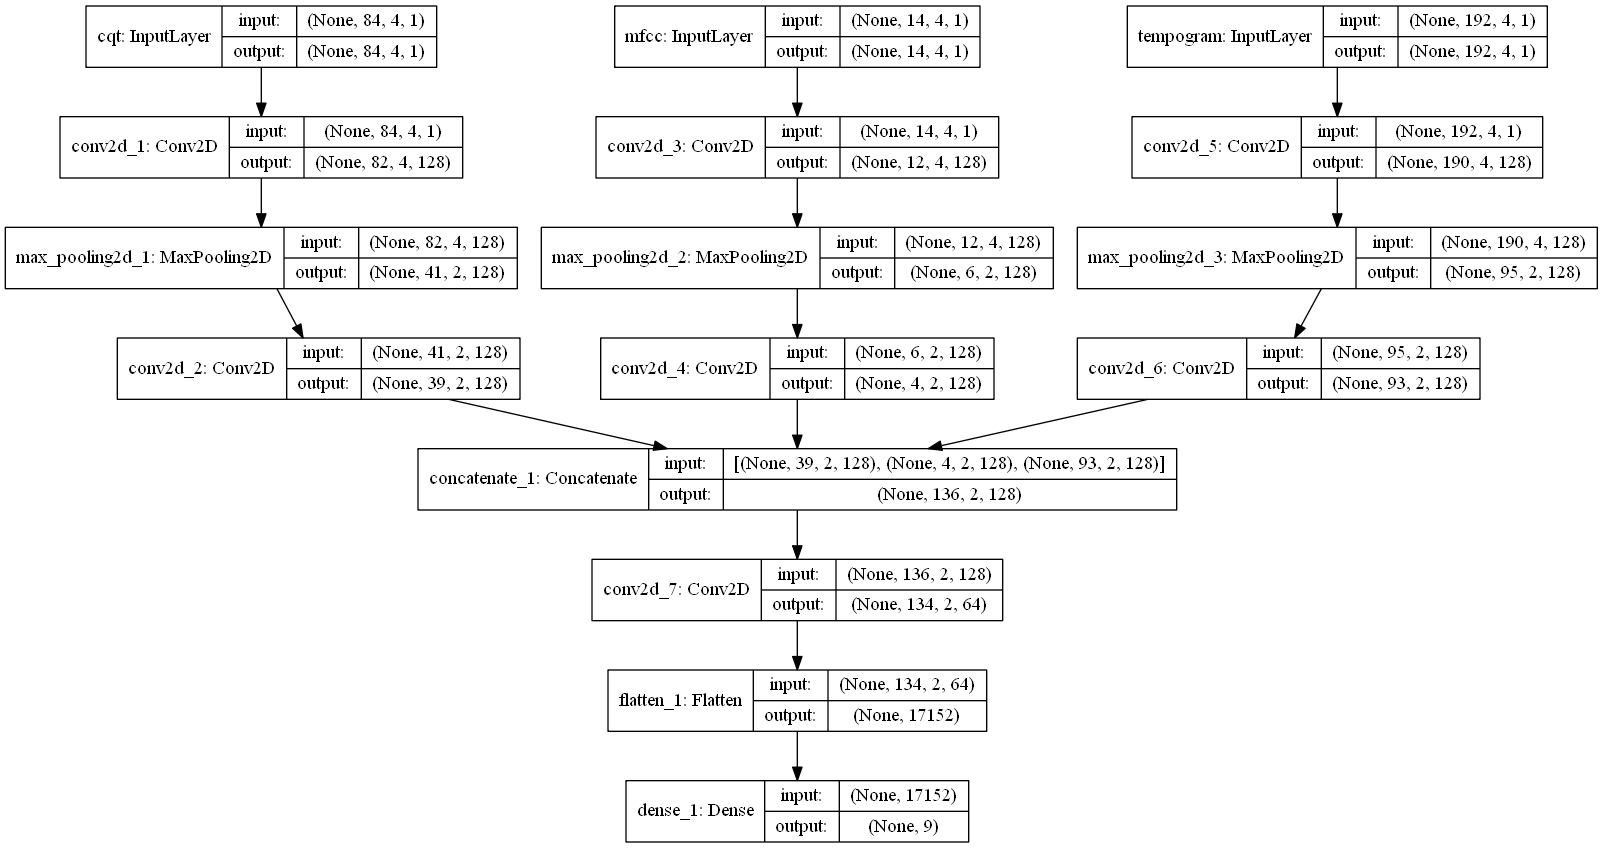
\includegraphics[width=1\textwidth]{images/cnn_architecture}
    \caption{Proposed CNN architecture with CQT, MFCC and Tempogram as example inputs.}
    \label{fig:proposed_cnn_architecture}
\end{figure}
Because of the great results with convolutional neural networks in the music structure analysis field, I propose an implementation of the segmentation approach using a convolutional neural network. 

This CNN has multiple input layers, one matrix per beat for each feature used. Each input matrix will therefore act as the input image, as described in the \nameref{sec:cnn_related} section. After each input layer there is a two-dimensional convolutional layer with a $3\times1$ kernel, followed by a possible two-dimensional max- or average-pooling layer with a $2\times2$ pooling size. Then another two-dimensional convolutional layer follows with 128 neurons and $3\times1$ kernel.

The outputs of this last convolutional layer of each input is then concatenated to one big $n\times4$ matrix. $n$ represents the summed length of the first dimension of each output shape. The concatenated outputs are then fed into a last two-dimensional convolutional layer, with 64 neurons and $3\times1$ kernel.

The (two-dimensional) output of the final convolutional layer is flattened into a single vector, and used as input for a dense layer with 9 neurons (each neuron representing one output label) and \textit{softmax} activation function. The softmax activation function normalizes the outputs of each neuron into a probability distribution, thus each output is scaled to be within the [0,1] interval and all scaled outputs sum to 1. The highest output is then selected as predicted label for the input, with its activation as confidence or probability that this label is the true label.

An example model, with CQT, MFCC and Tempogram as input features can be found in \autoref{fig:proposed_cnn_architecture}.

\subsection[Bi-LSTM]{Bi-Directional Long Short-Term Memory Artificial Neural Network}
\begin{figure}[t]
    \centering
    \begin{subfigure}{\textwidth}
        \centering
        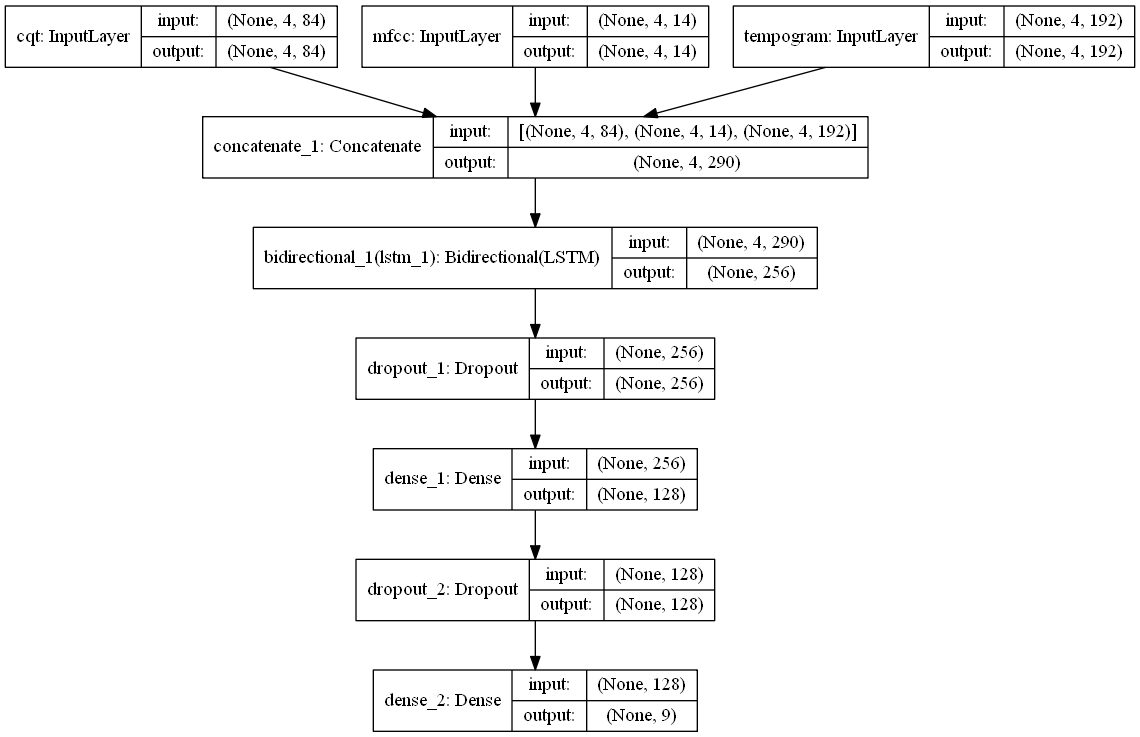
\includegraphics[width=.9\linewidth]{images/lstm_architecture_single}
        \caption{Single LSTM layer architecture.}
        \label{fig:lstm_single}
    \end{subfigure}
    \par\bigskip
    \begin{subfigure}{\textwidth}
        \centering
        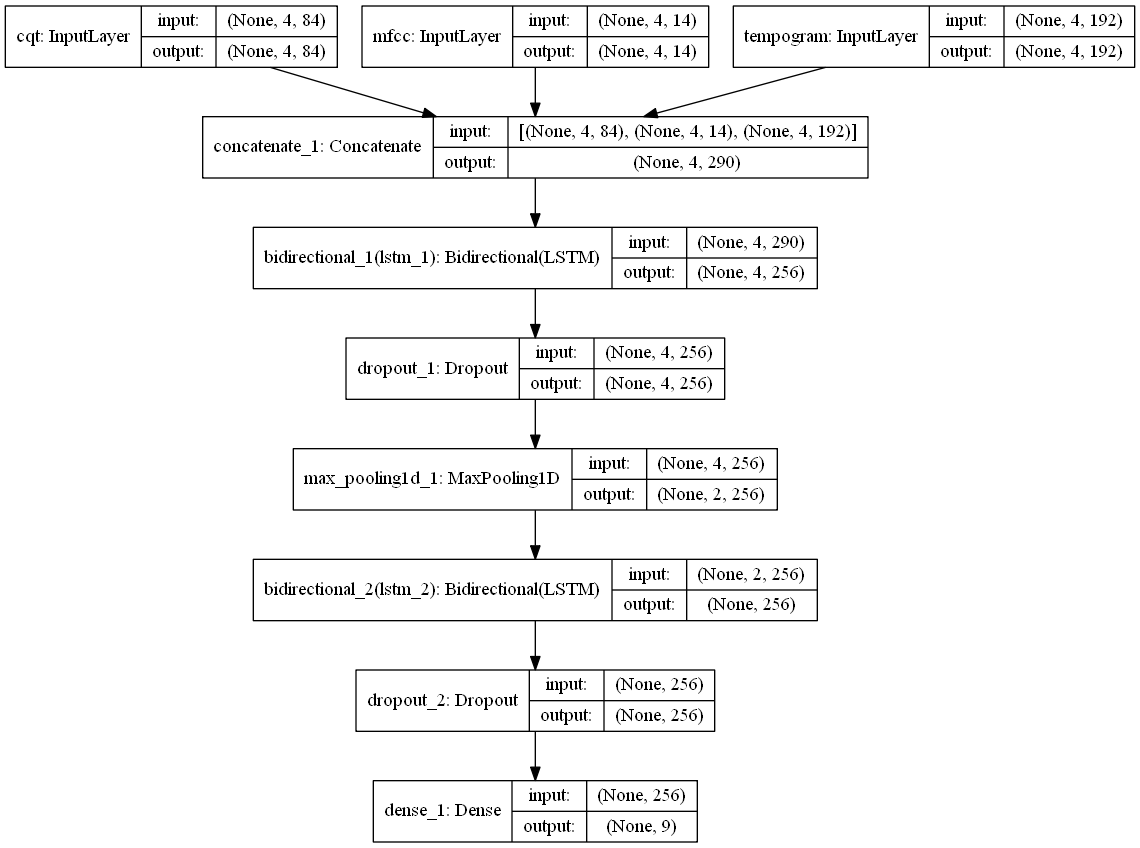
\includegraphics[width=.9\linewidth]{images/lstm_architecture_multi}
        \caption{Double LSTM layer architecture.}
        \label{fig:lstm_double}
    \end{subfigure}
    
    \caption{Proposed LSTM architectures with CQT, MFCC and Tempogram as example inputs.}
    \label{fig:proposed_lstm_architecture}
\end{figure}
Alongside a convolutional neural network, I also propose a bi-directional long short-term memory neural network implementation of the segmentation by annotation approach. This model will show if its capabilities to cope with temporal data and its performance in the automatic audio segmentation field also apply to music structure detection. The model is made bi-directional because of the reported increased performance of bi-directional recurrent neural networks over normal recurrent neural networks \cite{Schuster1997bidirectional}.

I propose two different architectures using long short-term memory units, a model with one bi-directional LSTM layer (\autoref{fig:lstm_single}), and a model with a double bi-directional LSTM layer, optionally combined with a max- or average-pooling layer (\autoref{fig:lstm_double}). Both models first contain an input layer per feature used, similar to the proposed CNN. In contrast to the CNN, all input is immediately concatenated into one matrix (with shape $n\times4$).

When a single LSTM layer model is build, this matrix is fed into bi-directional LSTM layer. However, since an (B-)LSTM layer has only one dimension, each column (or vector representing a beat) is separately evaluated. Because we want a single output from the full network, the B-LSTM layer is set to put one vector out after all 4 beats have been evaluated. This output is then passed into a dense layer, containing 128 neurons, whose output ultimately is put in a dense layer containing 9 neurons (each one representing one output label), and a \textit{softmax} activation function (\autoref{fig:lstm_single}).

If a double LSTM layer model is built the first B-LSTM layer does not first evaluate all 4 beats, but gives an output for each of the 4 beats. Each output is optionally passed through a one dimensional max- or average-pooling layer with a pool size of 2. Then another B-LSTM layer receives each output and evaluates all four, before outputting a single vector which is fed into the final dense layer with 9 neurons and softmax activation (\autoref{fig:lstm_double}).

\chapter{Experimental Results}
\label{ch:results}
In this chapter I report the initial results from the first test. After that I propose changes to this first test, and report the results from this final test.


\section{Evaluation Method}
\label{sec:eval_meth}
In order to find the best model on the dataset, I have created multiple models, each with different hyperparameters and combinations of features as input. I then tried to create a model for each possible combination of hyperparameters on each feature combination. Each model was created using the Keras \cite{Chollet2015keras} machine learning framework originally build for Python. This framework is build on top of the popular, well-known machine learning API \textit{Tensorflow 2.0} \cite{Tensorflow2015whitepaper}.

\subsection{The Hyperparameters}
\begin{table}[b]
    \centering
    \begin{tabular}{|l|l|}
    \hline
    \textbf{Hyperparameter} & \textbf{Values}                    \\ \hline\hline
    Neurons                 & 128, 256, 512                      \\ \hline
    Activation function     & \textit{ReLu, Elu}                 \\ \hline 
    Pooling                 & \textit{no\_pooling, max, average} \\ \hline
    Optimizer               & \textit{RMSprop, Adam}             \\ \hline
    Dropout                 & 10\%, 20\%, 30\%, 40\%, 50\%       \\ \hline
    Epochs                  & 1, 10, 50, 100                     \\ \hline
    Batch size              & 1, 5, 10, 50, 100                  \\ \hline
    \end{tabular}
    \caption{Initial hyperparameters and their initial range of values.}
    \label{tab:init_params}
\end{table}
For each generally important parameter for a neural network I've created a hyperparameter. I will explain each hyperparameter below. A list of all hyperparameters and their values can be found in \autoref{tab:init_params}.

\subsubsection{Neuron Count}
The first hyperparameter is the amount of neurons that make up the first layer, the first convolutional layer for the CNN models and the first or only B-LSTM layer of the LSTM models. I've chosen 128, 256 and 512 as possible neuron counts. 

\subsubsection{Activation Function}
\begin{figure}[t]
    \centering
    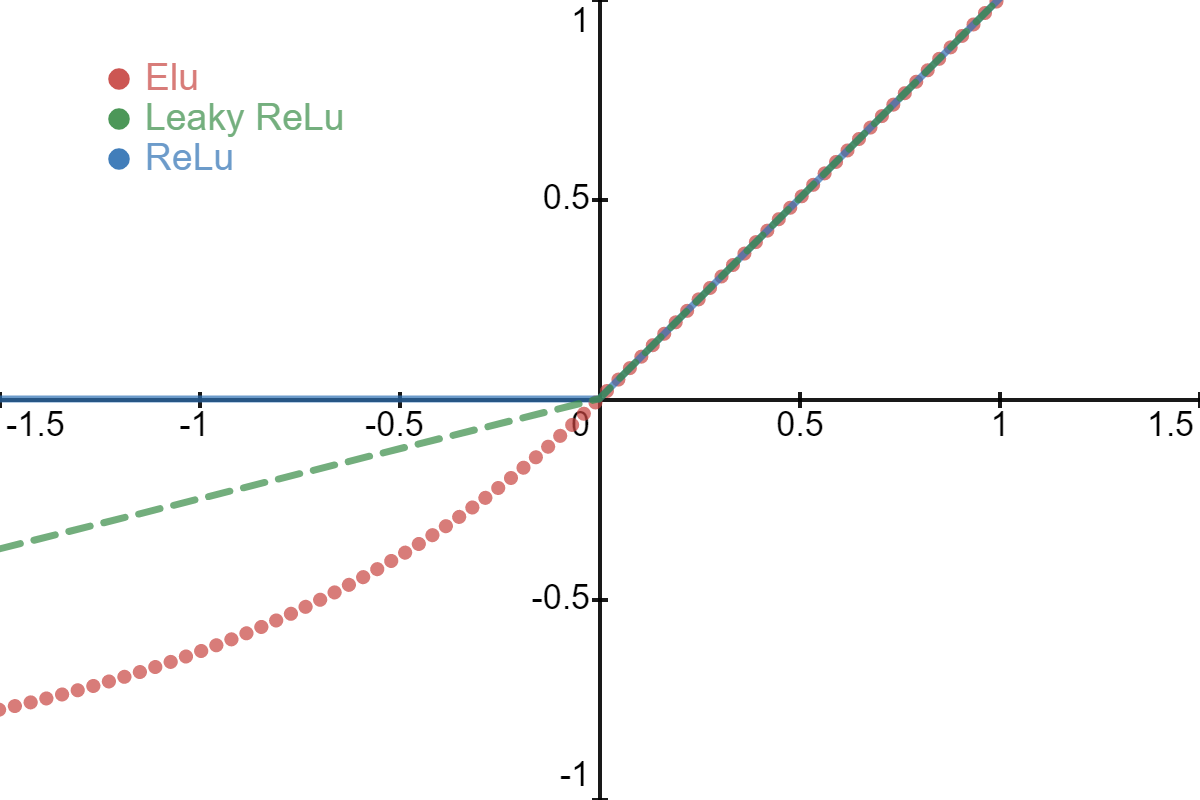
\includegraphics[width=.8\textwidth]{images/relu_elu-wide}
    \caption{Comparison of output of Elu, ReLu and Leaky ReLu activation functions on varying input values. If $x>0$, all activation functions have a linear output of $y=x$.}
    \label{fig:relu_elu}
\end{figure}
The second hyperparameter is the activation function of each neuron, the chosen activation function is applied on each layer, except for the final dense layer, which has a \textit{softmax} activation function (as explained in the \nameref{ch:method} chapter). I've included \textit{Rectified Linear Unit} (ReLu) \cite{Agarap2018deep} and \textit{Exponential Linear Unit} (Elu) as possible values. ReLu was included because it is seen as goto activation function, however because no negative activation is possible with this function, I've chosen to include Elu as activation function as well. Another alternative activation function close to ReLu allowing negative activation is Leaky ReLu, however this activation function was not available in Keras. A visualization of the different activation functions on varying input values can be found in \autoref{fig:relu_elu}.

\subsubsection{Pooling}
The output feature maps of convolutional layers are sensitive to the location of features in the input. One way of solving this problem is to down sample the feature maps. An approach to down sampling is provided in the form of a pooling layer. Two common types of pooling layers are defined: max and average. Max pooling works by returning the maximum value present in the pooling size as output, while average pooling works by calculating the average. The pooling layers defined in the models use local pooling with a pooling size of $2\times2$. 

Not only is pooling being used in convolutional networks, \textcite{Gimeno2020a} employ pooling between their bi-directional LSTM layers, that is why I have tested no pooling, max pooling and average pooling on both the CNN and LSTM models.

\subsubsection{Optimizer and Dropout}
Neural networks 'learn' by applying back propagation each learning iteration. During back propagation each weight is modified with regards to the output error. The aim is to reduce the value of the loss function. Because the models I created are multi-class classifiers with one true label, \textit{categorical cross entropy} is used as loss function in the models. Future research has to prove whether using other loss functions may be better instead \cite{Hsu2019multi}. To reduce the loss, the gradient is calculated. An optimizer is a function that can efficiently use this gradient to update the weights of the models to decrease the loss as fast as possible. One of the newest, most popular and best performing optimizers of this moment is the \textit{Adam} optimizer \cite{Kingma2014adam}. As comparison optimizer I've chosen the \textit{RMSprop} optimizer.

Another way of boosting the learning rate (or speed of which the loss decreases) is to use dropout. Dropout, introduced by \textcite{Hinton2012improving}, works by randomly 'dropping' a percentage of the neurons of certain layers. This means that all connections to these neurons are removed and that the other neurons are required to 'learn' the same representations that were first captured by the now removed neurons. Too low values for dropout are found to not have much impact, while too high dropout rates will reduce the overall performance of the models. 50\% dropout rate is generally seen as a the threshold from which the performance of the models will decrease, but still very much used \cite{Ullrich2014boundary}. I've therefore defined the set of dropout rates to range between 10\% and 50\% with a step size of 10\%. The dropout is applied on each layer except for the last dense layer.

\subsubsection{Epochs and Batch Size}
The final two parameters are used during the training phase of a model. These are the \textit{epochs} and \textit{batch size}. The amount of epochs defines how many times the training data is evaluated before the final model is returned. Increasing the amount of epochs means that the model has more time to learn all patterns into greater detail, however to high values will cause the model to overfit\footnote{If the model sees each sample many times it will become very good in classifying each sample, however new samples (less similar to the learned samples) will get a wrong classification more often.} and severely increases the time it takes to train the model. I've chosen to test models on 1, 10, 50 and 100 epochs (more epochs are being used in the field, this however would've made the training process all the much longer).

The batch size determines how many samples are passed through the network before back propagation is applied. The back propagation then is applied with the gradient of the loss of all these samples. Larger batch size generally speeds up the learning process of a model since less updates per epoch are performed. However, if the batch size is too large, a model will not always be able to learn specific patterns for one specific output, thus lowering its precision. I've chosen to create models with a wide range of batch size: 1, 5, 10, 50 and 100.

\subsubsection{Feature Combinations}
\begin{table}[t]
    \centering
    \begin{tabular}{|l|}
    \hline
    \textbf{Feature Combination}             \\ \hline\hline
    CQT, CENS, PCP, Tonnetz, MFCC, Tempogram \\ \hline
    CQT, MFCC                                \\ \hline
    CENS, MFCC                               \\ \hline
    PCP, MFCC                                \\ \hline
    Tonnetz, MFCC                            \\ \hline
    CQT, MFCC, Tempogram                     \\ \hline
    CENS, MFCC, Tempogram                    \\ \hline
    PCP, MFCC, Tempogram                     \\ \hline
    Tonnetz, MFCC, Tempogram                 \\ \hline
    CQT, Tempogram                           \\ \hline
    CENS, Tempogram                          \\ \hline
    PCP, Tempogram                           \\ \hline
    Tonnetz, Tempogram                       \\ \hline
    MFCC, Tempogram                          \\ \hline
    \end{tabular}
    \caption{Initial feature combinations.}
    \label{tab:init_feature_combo}
\end{table}
Based on previous research and type of each feature I've created 14 different sets of feature combinations, these can be found in \autoref{tab:init_feature_combo}. I've chosen to include a combination of all features extracted, combined with each feature paired with the MFCC, based on its overall high success rate in other research.

I've also included one a few of the possible chroma feature combined with one timbre feature combined with the tempogram combinations. To evaluate the performance of the tempogram I've included the pairing with each other feature to the feature combinations as well. The combinations missing are combinations of different timbre features and combinations of different chroma features, since combining a feature of one type with a feature of the same type will most likely not improve performance.

\subsubsection{Multi B-LSTM layer}
The LSTM models had one extra hyperparameter: whether to use a single or double B-LSTM layer. If a double LSTM layer model was made, and pooling was set to max or average, a pooling layer was put between the B-LSTM layers. Otherwise no pooling layer was used.


\section{Initial Test}
\subsection{Initial Test Setup}
 Using the possible values of each hyperparameter and the feature combinations an attempt had been made to create a model on each possible combination trained on 80\% of the total data (about 150000 samples) and evaluated on the remaining 20\% (35000). An output was registered of being correct when the index of neuron with the highest activation in the output layer corresponded with the index of the 1 in the one-hot-encoded true label vector and wrong otherwise. The accuracy was then calculated as the ratio of correct classifications to wrong classifications.

 One machine, containing an AMD Ryzen 7 3700x CPU and a NVIDIA GeForce GTX 1080 (8GB) GPU, was used to train and evaluate one CNN and one LSTM model simultaneously. Keras and the Tensorflow 2.0 backend were set to run on the GPU, while data flow was managed by the CPU.

\subsection{Initial Test Results}
Since both a CNN and LSTM model were trained simultaneously one epoch with a batch size of 1 roughly took $30\sim50$ seconds. A total of 50400 CNN models and 100800 LSTM models had to be trained. This means that about 6 million epochs of the data needed to be performed. Although only 20\% of the models have a batch size of 1, the expected time per epoch still was way above 10 seconds. This means that training and evaluating all CNN models would take 1 year and training all LSTM models around 2 years\footnote{Not counting the possible speedup when all CNN models have been evaluated. However, the very optimistic 10 seconds per epoch accounts for that.}.

Therefore the initial test setup was aborted after 1.5 weeks. In this time 145 LSTM and 292 CNN models were trained and evaluated. These models did not evaluate the impact of the amount of neurons, activation function and optimizer used nor the impact of the dropout. However, I was able to derive the impact of the amount of epochs, the batch size and feature combinations.

After preliminary data analysis, a number of trends were identified. The two trends that stood out the most were the amount of epochs and the batch size. A higher amount of epochs as well as a larger batch size always increased the performance of the model. The CQT turned out to be the best performing feature, with the Tempogram and MFCC being the two best features after that.   

The best performing CNN model had an accuracy of 0.66 on the test data, the best performing LSTM an accuracy of 0.43. No real performance increase of using a double B-LSTM layer over one B-LSTM layer was noticed.

\subsection{Adjustments}
To also be able to evaluate the other hyperparameter values, I made some changes to the search space.

\subsubsection{Feature Combinations}
\begin{table}[t]
    \centering
    \begin{tabular}{|l|}
    \hline
    \textbf{Feature Combination} \\ \hline\hline
    CQT, Tempogram               \\ \hline
    CQT, MFCC                    \\ \hline
    CQT, MFCC, Tempogram         \\ \hline
    \end{tabular}
    \caption{Final feature combinations.}
    \label{tab:final_feature_combo}
\end{table}
I first took a look at the feature combinations. The Tonnetz feature turned out to be too small of a feature to be usable with any pooling, and I therefore removed it from the features. Since no improvement was obtained using all features instead of only CQT, MFCC and Tempogram, the CENS and PCP features were removed from the feature combinations as well. This reduced the amount of feature combinations from 14 to 3. Thereby reducing the factor that determined the amount of models that had to be trained and evaluated the most. The final feature combinations can be found in \autoref{tab:final_feature_combo}.

\subsubsection{Hyperparameters}
After the feature combinations I've also reduced the amount of values of some hyperparameters. The most reduced ones are the epochs and batch size, these have been truncated to only contain 10, 50 and 100. Furthermore, I've reduced the dropout rates to 10\%, 25\% and 50\%. 

I've also trained the best performing CNN and LSTM on ReLu and Elu activation while using the Adam and RMSprop optimizer. This showed that using Elu did not improve the accuracy, while using the Adam optimizer heavily increased the accuracy with over 10\%. I therefore decided to use only ReLu as activation function and Adam optimizer as the only optimizer. As an additional benefit, Adam is a faster optimizer and therefore decreased the time of each epoch with quite a large factor. Furthermore, I removed the double B-LSTM layer hyperparameter, and chose to train only single B-LSTM layer models. The final hyperparameters and their values can be found in \autoref{tab:final_params}.

\subsubsection{Final Test}
\begin{table}[t]
    \centering
    \begin{tabular}{|l|l|}
    \hline
    \textbf{Hyperparameter} & \textbf{Values}                    \\ \hline\hline
    Neurons                 & 1285,256,512                       \\ \hline
    Activation function     & \textit{ReLu}                      \\ \hline
    Pooling                 & \textit{no\_pooling, max, average} \\ \hline
    Optimizer               & \textit{adam}                      \\ \hline
    Dropout                 & 10\%, 25\%, 50\%                   \\ \hline
    Epochs                  & 10, 50, 100                        \\ \hline
    Batch size              & 10, 50, 100                        \\ \hline
    \end{tabular}
    \caption{Final hyperparameters and their final range of values.}
    \label{tab:final_params}
\end{table}
One final big factor that increased the duration of each epoch was the amount of data. To decrease this heavy impacting factor, I've decided to take only 10\% of the original data as training and test data for the final test. The amount of samples used for training therefore decreased to 15000 and the amount of beats used for testing decreased to 3500. Although overall accuracy of the models were expected to be lower on this subset that on the full dataset, models with better hyperparameters and features will perform better than other models on both the full dataset or a subset thereof. Reducing the dataset too much can result in the training data not containing enough variation. I, however, expect 15000 samples to be quite representative for the full dataset, especially since all samples are chosen at random and not on a song basis. Each sample in this context means the concatenation of the feature vectors of the two beats before the current beat together with the feature vector of the current and the next beat.

The search space was now reduced to just above 700 different models. By using the Adam optimizer, removing the batch size of 1 and reducing the size of the dataset, the average time per epoch also reduced to around 3 seconds. The expected time to train and evaluate these models therefore reduced to less than a week, which was a lot more within the time-scope of this thesis. 


\section{Final Results}
% \begin{table}[t]
%     \centering
%     \begin{tabular}{|l|l|l|l|l|l|l|l|l|l|l|l|l|l|l|l|l|l|l|}
%     \hline
%                                                                                            & \multicolumn{3}{l|}{\textbf{Neuron Count}} & \multicolumn{3}{l|}{\textbf{Dropout}} & \multicolumn{3}{l|}{\textbf{Pooling}} & \multicolumn{3}{l|}{\textbf{Epochs}} & \multicolumn{3}{l|}{\textbf{Batch size}} & \multicolumn{3}{l|}{\textbf{Feature Combo}}                                                                                                                                         \\ \hline
%     \textbf{Values}                                                                        & 128          & 256          & 512          & 10\%        & 25\%       & 50\%       & none      & max        & average      & 10        & 50          & 100        & 10           & 50          & 100         & \begin{tabular}[c]{@{}l@{}}CQT +\\ Tempogram\end{tabular} & \begin{tabular}[c]{@{}l@{}}CQT +\\ MFCC\end{tabular} & \begin{tabular}[c]{@{}l@{}}CQT + MFCC +\\ Tempogram\end{tabular} \\ \hline
%     \textbf{\begin{tabular}[c]{@{}l@{}}Amount of models\\ created with value\end{tabular}} & 267          & 250          & 218          & 316         & 232        & 187        & 242       & 259        & 234          & 255       & 244         & 236        & 249          & 245         & 241         & 202                                                       & 201                                                  & 200                                                              \\ \hline
%     \textbf{\begin{tabular}[c]{@{}l@{}}Amount of models \\ in top 10\%\end{tabular}}       & 37           & 18           & 15           & 27          & 28         & 15         & 0         & 43         & 27           & 0         & 20          & 50         & 2            & 27          & 41          & 37                                                        & 0                                                    & 18                                                               \\ \hline
%     \textbf{\begin{tabular}[c]{@{}l@{}}Percentage of models\\ in top 10\%\end{tabular}}    & 0.139        & 0.072        & 0.069        & 0.085       & 0.121      & 0.080      & 0         & 0.166      & 0.115        & 0         & 0.082       & 0.212      & 0.008        & 0.110       & 0.170       & 0.183                                                     & 0                                                    & 0.090                                                            \\ \hline
%     \end{tabular}
%     \caption{Analysis of all models created with different parameter values and feature combinations}
%     \label{tab:model_analysis}
% \end{table}


% \begin{table}[t]
%     \centering
%     \begin{tabular}{|l||l|l|l|l|}
%     \hline
%                                             & \textbf{Values}                                                  & \textbf{\begin{tabular}[c]{@{}l@{}}No. models\\ created with value\end{tabular}} & \textbf{\begin{tabular}[c]{@{}l@{}}No. models\\in top 10\%\end{tabular}} & \textbf{\begin{tabular}[c]{@{}l@{}}\%. models\\in top 10\%\end{tabular}} \\ \hline\hline
%     \multirow{3}{*}{\textbf{Neuron\\Count}}  & 128                                                              & 267                                                                                    & 37                                                                               & \textbf{0.139}                                                                      \\ \cline{2-5} 
%                                             & 256                                                              & 250                                                                                    & 18                                                                               & 0.072                                                                               \\ \cline{2-5} 
%                                             & 512                                                              & 218                                                                                    & 15                                                                               & 0.069                                                                               \\ \hline
%     \multirow{3}{*}{\textbf{Dropout}}       & 10\%                                                             & 316                                                                                    & 27                                                                               & 0.085                                                                               \\ \cline{2-5} 
%                                             & 25\%                                                             & 232                                                                                    & 28                                                                               & \textbf{0.121}                                                                      \\ \cline{2-5} 
%                                             & 50\%                                                             & 187                                                                                    & 15                                                                               & 0.080                                                                               \\ \hline
%     \multirow{3}{*}{\textbf{Pooling}}       & none                                                             & 242                                                                                    & 0                                                                                & 0                                                                                   \\ \cline{2-5} 
%                                             & max                                                              & 259                                                                                    & 43                                                                               & \textbf{0.166}                                                                      \\ \cline{2-5} 
%                                             & average                                                          & 234                                                                                    & 27                                                                               & 0.115                                                                               \\ \hline
%     \multirow{3}{*}{\textbf{Epochs}}        & 10                                                               & 255                                                                                    & 0                                                                                & 0                                                                                   \\ \cline{2-5} 
%                                             & 50                                                               & 244                                                                                    & 20                                                                               & 0.082                                                                               \\ \cline{2-5} 
%                                             & 100                                                              & 236                                                                                    & 50                                                                               & \textbf{0.212}                                                                      \\ \hline
%     \multirow{3}{*}{\textbf{Batch\\size}}    & 10                                                               & 249                                                                                    & 2                                                                                & 0.008                                                                               \\ \cline{2-5} 
%                                             & 50                                                               & 245                                                                                    & 27                                                                               & 0.110                                                                               \\ \cline{2-5} 
%                                             & 100                                                              & 241                                                                                    & 41                                                                               & \textbf{0.170}                                                                      \\ \hline
%     \multirow{3}{*}{\textbf{Feature\\Combo}} & \begin{tabular}[c]{@{}l@{}}CQT +\\ Tempogram\end{tabular}        & 202                                                                                    & 37                                                                               & \textbf{0.183}                                                                      \\ \cline{2-5} 
%                                             & \begin{tabular}[c]{@{}l@{}}CQT +\\ MFCC\end{tabular}             & 201                                                                                    & 0                                                                                & 0                                                                                   \\ \cline{2-5} 
%                                             & \begin{tabular}[c]{@{}l@{}}CQT + MFCC +\\ Tempogram\end{tabular} & 200                                                                                    & 18                                                                               & 0.090                                                                               \\ \hline
%     \end{tabular}
% \end{table}

% Please add the following required packages to your document preamble:
% \usepackage{multirow}
\begin{table}[t]
    \centering
    \begin{tabular}{|l||l|l|l|l|}
    \hline
                                                                                       & \textbf{Values}                                                  & \textbf{\begin{tabular}[c]{@{}l@{}}No. models\\ created\end{tabular}} & \textbf{\begin{tabular}[c]{@{}l@{}}No. models \\ in top 10\%\end{tabular}} & \textbf{\begin{tabular}[c]{@{}l@{}}\%. models\\ in top 10\%\end{tabular}} \\ \hline\hline
    \multirow{3}{*}{\textbf{\begin{tabular}[c]{@{}l@{}}Neuron \\ Count\end{tabular}}}  & 128                                                              & 267                                                                   & 37                                                                         & \textbf{0.139}                                                            \\ \cline{2-5} 
                                                                                       & 256                                                              & 250                                                                   & 18                                                                         & 0.072                                                                     \\ \cline{2-5} 
                                                                                       & 512                                                              & 218                                                                   & 15                                                                         & 0.069                                                                     \\ \hline\hline
    \multirow{3}{*}{\textbf{Dropout}}                                                  & 10\%                                                             & 316                                                                   & 27                                                                         & 0.085                                                                     \\ \cline{2-5} 
                                                                                       & 25\%                                                             & 232                                                                   & 28                                                                         & \textbf{0.121}                                                            \\ \cline{2-5} 
                                                                                       & 50\%                                                             & 187                                                                   & 15                                                                         & 0.080                                                                     \\ \hline\hline
    \multirow{3}{*}{\textbf{Pooling}}                                                  & none                                                             & 242                                                                   & 0                                                                          & 0                                                                         \\ \cline{2-5} 
                                                                                       & max                                                              & 259                                                                   & 43                                                                         & \textbf{0.166}                                                            \\ \cline{2-5} 
                                                                                       & average                                                          & 234                                                                   & 27                                                                         & 0.115                                                                     \\ \hline\hline
    \multirow{3}{*}{\textbf{Epochs}}                                                   & 10                                                               & 255                                                                   & 0                                                                          & 0                                                                         \\ \cline{2-5} 
                                                                                       & 50                                                               & 244                                                                   & 20                                                                         & 0.082                                                                     \\ \cline{2-5} 
                                                                                       & 100                                                              & 236                                                                   & 50                                                                         & \textbf{0.212}                                                            \\ \hline\hline
    \multirow{3}{*}{\textbf{\begin{tabular}[c]{@{}l@{}}Batch \\ size\end{tabular}}}    & 10                                                               & 249                                                                   & 2                                                                          & 0.008                                                                     \\ \cline{2-5} 
                                                                                       & 50                                                               & 245                                                                   & 27                                                                         & 0.110                                                                     \\ \cline{2-5} 
                                                                                       & 100                                                              & 241                                                                   & 41                                                                         & \textbf{0.170}                                                            \\ \hline\hline
    \multirow{3}{*}{\textbf{\begin{tabular}[c]{@{}l@{}}Feature \\ Combo\end{tabular}}} & \begin{tabular}[c]{@{}l@{}}CQT +\\ Tempogram\end{tabular}        & 202                                                                   & 37                                                                         & \textbf{0.183}                                                            \\ \cline{2-5} 
                                                                                       & \begin{tabular}[c]{@{}l@{}}CQT +\\ MFCC\end{tabular}             & 201                                                                   & 0                                                                          & 0                                                                         \\ \cline{2-5} 
                                                                                       & \begin{tabular}[c]{@{}l@{}}CQT + MFCC +\\ Tempogram\end{tabular} & 200                                                                   & 18                                                                         & 0.090                                                                     \\ \hline
    \end{tabular}
    \caption{Analysis of all CNN models created with different parameter values and feature combinations. Best performing value of each parameter had been put in bold.}
    \label{tab:model_analysis}
\end{table}
After 5 days all models were trained and evaluated. The accuracy of each model was saved in a text file, named by the parameter values and features used to create that model separated by an underscore. All models were then grouped in a list sorted by their accuracy in descending order. I analysed each parameter by grouping all models by their value for that parameter. Then I counted the total amount of models made with that value for the parameter and amount of models in the top 10\% of all models (around 700 models were created, top 10\% therefore accounted for 70 models). With these counts I calculated the percentage of models with that value in the top 10\% of models. This gives a distribution of best performing parameter value on the top 30\% of all models. All distributions can be found in \autoref{tab:model_analysis}.

Using the percentages, a best performing value for each parameter can be derived. This does not immediately mean that the best performing models has these values for each parameter, however further analysis showed that the model with these parameter values and feature combination as input, indeed was among the top 3 best performing models. 

\subsection{Best performing CNN and LSTM models}
\subsubsection{Parameter values and input features combination}
Following the analysis of the parameter values, I've defined the best performing CNN and LSTM models. These models both have a neuron count of 128 in the first layer, a dropout of 25\%, max pooling, a batch size and epoch count of 100, ReLu activation function and Adam optimizer. As input features I've chosen the Constant-Q Transform in combination with the Tempogram. Using the best performing values for each parameter together with all features as input only improved the accuracy with $<1$\%, while increasing evaluation time. The LSTM model has only one B-LSTM layer, since adding more layers did not improve its accuracy but instead added more time to the training and evaluation time of the model.

\subsubsection{Evaluation of best models on different datasets}
% \begin{table}[t]    
%     \begin{tabular}{lll}
%                       & CNN    & LSTM   \\
%     Training Accuracy & 0.9456 & 0.8265 \\
%     Test Accuracy     & 0.80   & 0.77   \\
%     1200 Accuracy     & 0.89   & 0.84  
%     \end{tabular}
%     \label{tab:final_results}
% \end{table}

%%%%%%%%%%%%%%%%%%
% Too wide table %
%%%%%%%%%%%%%%%%%%
% \begin{table}[t]
%     \centering
%     \begin{tabular}{|l|l|l|l|l|l|l|l|l|l|l|l|}
%     \hline
%     \multirow{2}{*}{}              & \multicolumn{2}{l|}{\textbf{Beat Classification Accuracy}} & \multirow{2}{*}{} & \multicolumn{2}{l|}{\textbf{\begin{tabular}[c]{@{}l@{}}All songs own\\ ground truth\end{tabular}}} & \multicolumn{2}{l|}{\textbf{\begin{tabular}[c]{@{}l@{}}All songs SALAMI\\ ground truth\end{tabular}}} & \multicolumn{2}{l|}{\textbf{\begin{tabular}[c]{@{}l@{}}SALAMI song-id 1200 own\\ ground truth\end{tabular}}} & \multicolumn{2}{l|}{\textbf{\begin{tabular}[c]{@{}l@{}}SALAMI song-id 1200 SALAMI\\ ground truth\end{tabular}}} \\ \cline{2-3} \cline{5-12} 
%                                    & Training data                 & Test data                  &                   & Non-Trimmed                                        & Trimmed                                       & Non-Trimmed                                         & Trimmed                                         & Non-Trimmed                                             & Trimmed                                            & Non-Trimmed                                              & Trimmed                                              \\ \hline
%     \multirow{2}{*}{\textbf{CNN}}  & \multirow{2}{*}{0.9456}       & \multirow{2}{*}{0.80}      & 0.5F              & 0.6849                                             & 0.5627                                        & 0.1451                                              & 0.0374                                          & 0.6087                                                  & 0.5261                                             & 0.55                                                     & 0.48                                                 \\ \cline{4-12} 
%                                    &                               &                            & 3F                & 0.8545                                             & 0.7935                                        & 0.3397                                              & 0.1960                                          & 0.9565                                                  & 0.9474                                             & 0.69                                                     & 0.64                                                 \\ \hline
%     \multirow{2}{*}{\textbf{LSTM}} & \multirow{2}{*}{0.8265}       & \multirow{2}{*}{0.77}      & 0.5F              & 0.4526                                             & 0.3003                                        & 0.1474                                              & 0.0581                                          & 0.3846                                                  & 0.2727                                             & 0.38                                                     & 0.29                                                 \\ \cline{4-12} 
%                                    &                               &                            & 3F                & 0.6141                                             & 0.5065                                        & 0.3487                                              & 0.2296                                          & 0.6923                                                  & 0.6364                                             & 0.56                                                     & 0.50                                                 \\ \hline
%     \end{tabular}
%     \caption{Final Results}
%     \label{tab:final_results}
% \end{table}

% Please add the following required packages to your document preamble:
% \usepackage{multirow}
\begin{table}[t]
    \centering
    \begin{tabular}{|l|l||l|l|l|l|}
    \hline
                                                                                             \textbf{Dataset} & \textbf{Measure} & \multicolumn{2}{l|}{\textbf{CNN}} & \multicolumn{2}{l|}{\textbf{LSTM}} \\ \hline\hline
    \multirow{2}{*}{\textbf{\begin{tabular}[c]{@{}l@{}}Beat Classification \\ Accuracy\end{tabular}}}            & Training data & \multicolumn{2}{l|}{0.9456}       & \multicolumn{2}{l|}{0.8265}        \\ \cline{2-6} 
                                                                                                                 & Test data     & \multicolumn{2}{l|}{0.80}         & \multicolumn{2}{l|}{0.77}          \\ \hline\hline
    \multicolumn{2}{|l|}{}                                                                                                       & \textbf{0.5F}   & \textbf{3F}     & \textbf{0.5F}    & \textbf{3F}     \\ \hline
    \multirow{2}{*}{\textbf{\begin{tabular}[c]{@{}l@{}}All songs \\ own ground truth\end{tabular}}}              & Untrimmed   & 0.6849          & 0.8545          & 0.4526           & 0.6141          \\ \cline{2-6} 
                                                                                                                 & Trimmed       & 0.5627          & 0.7935          & 0.3003           & 0.5065          \\ \hline
    \multirow{2}{*}{\textbf{\begin{tabular}[c]{@{}l@{}}All songs \\ SALAMI ground truth\end{tabular}}}           & Untrimmed   & 0.1451          & 0.3397          & 0.1474           & 0.3487          \\ \cline{2-6} 
                                                                                                                 & Trimmed       & 0.0374          & 0.1960          & 0.0581           & 0.2296          \\ \hline
    \multirow{2}{*}{\textbf{\begin{tabular}[c]{@{}l@{}}SALAMI song-id 1200 \\ own ground truth\end{tabular}}}    & Untrimmed   & 0.6087          & 0.9565          & 0.3846           & 0.6923          \\ \cline{2-6} 
                                                                                                                 & Trimmed       & 0.5261          & 0.9474          & 0.2727           & 0.6364          \\ \hline
    \multirow{2}{*}{\textbf{\begin{tabular}[c]{@{}l@{}}SALAMI song-id 1200 \\ SALAMI ground truth\end{tabular}}} & Untrimmed   & 0.55            & 0.69            & 0.38             & 0.56            \\ \cline{2-6} 
                                                                                                                 & Trimmed       & 0.48            & 0.64            & 0.29             & 0.50            \\ \hline
    \end{tabular}
    \caption{An overview of the final CNN and LSTM model evaluated on multiple datasets. The training- and testset accuracy is evaluated using Keras. The F-measures on SALAMI 1200 (custom and original ground truth) as well as the F-measures on the full SALAMI dataset (custom and original ground truth) are calculated using the MSAF. In all cases the same CNN or LSTM model were used, these are the ones trained on the custom ground truth (9 unique output labels).} 
    \label{tab:final_results}
\end{table}
I then trained each best model on the full dataset, with 80\% of the dataset as training data and the remaining 20\% as test data. The accuracy on the training and test data were 94.56\% and 80\% for the CNN model and 82.65\% and 77\% for the LSTM model respectively (\autoref{tab:final_results} first row). These models were then saved in \textit{.h5} file. This file format is used by Keras to models with their trained weights. This way inference can be easily applied on another machine, since the model only needs to be loaded instead of fully trained\footnote{It can also be used to further train the network on other or more data on another machine and than re-saved as \textit{.h5} file, however this is less common in practice.}.

Since the end goal was to segment a song into \textit{chorus}, \textit{verse}, etc. instead of predicting a single beat, I've taken a few arbitrary songs from the dataset. Then I looked at the amount of segments and the amount of different labels. Based on this I've taken SALAMI song-id 1200 as my test song for the final models. To perform the test I've sequentially inferred the label of each beat of the song with each model. As expected there were some beats that had another label than the labels of a number of beats around it. This is due to the less than 100\% accuracy of the models on the dataset (which is to be desired, since they would be overfitted otherwise). 

\subsubsection{Label Filtering Function}
\begin{table}[t]
    \centering
    \begin{tabular}{|l|l|l|l|l|}
    \hline
    \textbf{Beat} & \textbf{Beat Start Time} & \textbf{True Label} & \textbf{Predicted Label} & \textbf{Filtered Label} \\ \hline\hline
    0             & 1.253877551020408  & no\_function        & no\_function             & no\_function            \\ \hline
    1             & 1.764716553287982  & no\_function        & no\_function             & no\_function            \\ \hline
    2             & 2.321995464852609  & no\_function        & no\_function             & no\_function            \\ \hline
    3             & 2.832834467120181  & no\_function        & no\_function             & no\_function            \\ \hline
    4             & 3.390113378684807  & no\_function        & no\_function             & no\_function            \\ \hline
    5             & 3.900952380952381  & intro               & intro                    & intro                   \\ \hline
    6             & 4.458231292517007  & intro               & intro                    & intro                   \\ \hline
    7             & 4.96907029478458   & intro               & intro                    & intro                   \\ \hline
    8             & 5.479909297052155  & intro               & intro                    & intro                   \\ \hline
    9             & 6.03718820861678   & intro               & intro                    & intro                   \\ \hline
    10            & 6.548027210884354  & intro               & intro                    & intro                   \\ \hline
    11            & 7.058866213151927  & intro               & intro                    & intro                   \\ \hline
    12            & 7.569705215419501  & intro               & verse                    & intro                   \\ \hline
    13            & 8.080544217687075  & intro               & intro                    & intro                   \\ \hline
    14            & 8.591383219954649  & intro               & solo                     & intro                   \\ \hline
    15            & 9.102222222222222  & intro               & intro                    & intro                   \\ \hline
    \dots         & \dots              & \dots               & \dots                    & \dots                   \\ \hline
    \dots         & \dots              & \dots               & \dots                    & \dots                   \\ \hline
    \dots         & \dots              & \dots               & \dots                    & \dots                   \\ \hline
    453           & 238.3760544217687  & solo                & solo                     & solo                    \\ \hline
    454           & 238.8868934240363  & solo                & solo                     & solo                    \\ \hline
    455           & 239.3977324263039  & solo                & no\_function             & solo                    \\ \hline
    456           & 239.9085714285714  & solo                & solo                     & solo                    \\ \hline
    457           & 240.419410430839   & solo                & solo                     & solo                    \\ \hline
    458           & 240.9302494331066  & solo                & solo                     & solo                    \\ \hline
    459           & 241.4410884353742  & solo                & solo                     & solo                    \\ \hline
    460           & 241.9519274376417  & solo                & solo                     & solo                    \\ \hline
    461           & 242.4627664399093  & solo                & solo                     & solo                    \\ \hline
    462           & 242.9271655328798  & solo                & chorus                   & solo                    \\ \hline
    463           & 243.3915646258504  & solo                & chorus                   & solo                    \\ \hline
    464           & 243.8559637188209  & solo                & solo                     & solo                    \\ \hline
    465           & 244.3668027210885  & solo                & solo                     & solo                    \\ \hline
    466           & 244.8776417233560  & solo                & solo                     & solo                    \\ \hline
    467           & 245.3884807256236  & solo                & solo                     & solo                    \\ \hline
    468           & 245.8528798185941  & solo                & no\_function             & solo                    \\ \hline
    \end{tabular}
    \caption{First and last 50 beats of SALAMI 1200 true, predicted and filtered labels produced by best CNN model.}
    \label{tab:1200_cnn}
\end{table}
\begin{table}[t]
    \centering
    \begin{tabular}{|l|l|l|l|l|}
    \hline
    \textbf{Beat}        & \textbf{Beat Start Time}   & \textbf{True Label}  & \textbf{Predicted Label} & \textbf{Filtered Label} \\ \hline\hline
    0                    & 1.25387755102041     & no\_function         & no\_function             & no\_function            \\ \hline
    1                    & 1.764716553287982    & no\_function         & no\_function             & no\_function            \\ \hline
    2                    & 2.321995464852608    & no\_function         & no\_function             & no\_function            \\ \hline
    3                    & 2.832834467120181    & no\_function         & no\_function             & no\_function            \\ \hline
    4                    & 3.390113378684807    & no\_function         & no\_function             & no\_function            \\ \hline
    5                    & 3.900952380952381    & intro                & no\_function             & no\_function            \\ \hline
    6                    & 4.458231292517007    & intro                & intro                    & intro                   \\ \hline
    7                    & 4.96907029478458     & intro                & intro                    & intro                   \\ \hline
    8                    & 5.479909297052155    & intro                & intro                    & intro                   \\ \hline
    9                    & 6.03718820861678     & intro                & intro                    & intro                   \\ \hline
    10                   & 6.548027210884354    & intro                & intro                    & intro                   \\ \hline
    11                   & 7.058866213151927    & intro                & intro                    & intro                   \\ \hline
    12                   & 7.569705215419501    & intro                & intro                    & intro                   \\ \hline
    13                   & 8.080544217687075    & intro                & intro                    & intro                   \\ \hline
    14                   & 8.591383219954649    & intro                & intro                    & intro                   \\ \hline
    15                   & 9.102222222222222    & intro                & intro                    & intro                   \\ \hline
    \dots                & \dots                & \dots                & \dots                    & \dots                   \\ \hline
    \dots                & \dots                & \dots                & \dots                    & \dots                   \\ \hline
    \dots                & \dots                & \dots                & \dots                    & \dots                   \\ \hline
    453                  & 238.3760544217687    & solo                 & solo                     & solo                    \\ \hline
    454                  & 238.8868934240363    & solo                 & solo                     & solo                    \\ \hline
    455                  & 239.3977324263039    & solo                 & solo                     & solo                    \\ \hline
    456                  & 239.9085714285714    & solo                 & solo                     & solo                    \\ \hline
    457                  & 240.419410430839     & solo                 & solo                     & solo                    \\ \hline
    458                  & 240.9302494331066    & solo                 & solo                     & solo                    \\ \hline
    459                  & 241.4410884353742    & solo                 & solo                     & solo                    \\ \hline
    460                  & 241.9519274376417    & solo                 & chorus                   & solo                    \\ \hline
    461                  & 242.4627664399093    & solo                 & solo                     & solo                    \\ \hline
    462                  & 242.9271655328798    & solo                 & solo                     & solo                    \\ \hline
    463                  & 243.3915646258504    & solo                 & solo                     & solo                    \\ \hline
    464                  & 243.8559637188209    & solo                 & solo                     & solo                    \\ \hline
    465                  & 244.3668027210885    & solo                 & solo                     & solo                    \\ \hline
    466                  & 244.8776417233560    & solo                 & verse                    & solo                    \\ \hline
    467                  & 245.3884807256236    & solo                 & solo                     & solo                    \\ \hline
    468                  & 245.8528798185941    & solo                 & chorus                   & solo                    \\ \hline
    \end{tabular}
    \caption{First and last 15 beats of SALAMI 1200 true, predicted and filtered labels produced by best LSTM model.}
    \label{tab:1200_lstm}
\end{table}
To still be able to use the start of a sequence of new labels as start of a segment I wrote a simple filtering function, based on the predictions on SALAMI 1200. This functions works by iterating over all the predicted labels of the beats. When a label different to the label of the beat before it is detected, the next 4 beats are scanned. If the label of the previous beat is detected in the labels of the next 4 beats, that label is taken as filtered label, otherwise the predicted label is taken as filtered label. This function thus requires each segment to be at least 5 beats in length, which is quite common in the ground truth I created based on the label grouping mentioned in \nameref{sec:3.the_data} section in \autoref{ch:method}. In the SALAMI dataset this is less common, but I will elaborate on this in the \nameref{ch:discussion} chapter.

I have also tried another filtering function. This function worked similar to the filtering function I used, however instead of checking if the label of the previous beat occurs in the labels of the next 4 beats, the most occurring label of the next 5 beats was taken as filtered label. The problem of this function was that if there were 3 falsely classified beats among the next 5 beats, this was taken as filtered label, thus causing a short, falsely classified segment to occur in the filtered predictions. This function also required segments of at least 6 beats, 1 beat (about 0.5 seconds) longer than the other filtering function, which can already be quite impactful.\\

The ground truth, predicted and filtered output of the CNN model on the first and last 15 beats of SALAMI 1200 can be found in \autoref{tab:1200_cnn}, the same output of the LSTM model on the first and last 15 beats of SALAMI 1200 can be found in \autoref{tab:1200_lstm}.

\subsubsection{Final Evaluation on SALAMI and own Ground Truth}
Using the filtering function I described earlier, I was able to create a \textit{JSON Annotated Music Specification} (JAMS) file \cite{Humphrey2014jams} of each song from the dataset. I also created a JAMS file for each ground truth I created. I then used the Music Structure Analysis Framework (MSAF) \cite{Nieto2016systematic} to evaluate the filtered segments of the CNN and LSTM models on both the SALAMI and my own ground truths.

The MSAF returns quite an extensive evaluation report. To enhance overview, I have only included the (mean) F-measures from the reports. Four different F-measures are returned with each report. An F-measure of an evaluation of the segment boundary location with a 0.5 second and 3 seconds time tolerance to the ground truth, both trimmed and untrimmed. MSAF automatically adds a segment boundary at the start and end of a song, if the untrimmed F-measure is calculated, these segment boundaries are included in the calculation. If a trimmed F-measure is calculated, these segment boundaries are excluded from the calculation, often lowering the F-measure, since only the segment boundaries produced by the models are now taken into account.

All F-measures can be found in \autoref{tab:final_results}, the full ground truth, predicted and filtered labels of SALAMI 1200 of the CNN \href{https://git.science.uu.nl/l.m.vanboven/bachelor-scriptie-musical-sctructure-analysis/-/blob/master/Leander/Results_Analysis/1200_cnn.csv}{here (link)}, and the same data of the LSTM \href{https://git.science.uu.nl/l.m.vanboven/bachelor-scriptie-musical-sctructure-analysis/-/blob/master/Leander/Results_Analysis/1200_lstm.csv}{here (link)}.

\chapter{Discussion}
\label{ch:discussion}
The focus of this chapter is to interpret the results reported in the previous chapter. After this interpretation a discussion of the results is held. The different architectures are compared to each other as well will the SbA approach be compared to the DSA approach to MSA. These comparisons aim to provide an answer to the research questions.


\section{Results Evaluation}
\subsubsection{Beat Classification Accuracy}
Looking at the absolute performance of the best CNN and LSTM model on classifying a beat, one may conclude that the convolutional model performs better than the long short-term memory model. However, looking at the accuracy of both models on the training and test data, the CNN model drops relatively more in accuracy (15.4\% for the CNN, 6.8\% for the LSTM). This may be an indication of the CNN model being overfit on the training data, therefore reducing its capabilities of classifying beats that the model has not 'seen' before. The possible overfit is unlikely to be a result of too little data since the LSTM did not seem to overfit on the data. The relatively small drop in accuracy for the LSTM model going from the training data to the test data may also indicate that the LSTM managed to capture the overall patterns that define the label of a certain beat, although less accurate for this particular set of beats.

\subsection{Segment Boundary Detection Accuracy}
When looking at the results of the JAMS files with the filtered labels evaluated by the MSAF, we need to take them with a grain of salt. There are a few reasons for this.

\subsubsection{Own ground truth}
Although the models have been trained and evaluated on the ground truth I created, MSAF only evaluates the accuracy of locating the segment boundary locations of each model. The accuracy is therefore not only subject to the pure performance of a model to classify a beat, but also to the performance of the filtering function. Since I primarily focused on the first, the latter received way less to none effort. As described in \autoref{ch:results}, the filtering function was based on the predictions made on SALAMI 1200, and the function was therefore optimized to generate filtered labels, and therefore segment boundaries that would make sense, for this specific song. We see that this indeed is the case, since the trimmed and untrimmed F-measures, with 3 seconds tolerance, on SALAMI 1200 (own ground truth) far exceeds the trimmed and untrimmed 3 second F-measure on the full dataset (own ground truth).

It is, however, interesting that the trimmed and untrimmed 0.5 second F-measure on SALAMI 1200 (own ground truth) is lower than the same F-measure on the full dataset (own ground truth) for both the CNN and LSTM model. We see that both the trimmed and untrimmed F-measures severely drop going from a 3 second tolerance to a 0.5 second tolerance (25\% to 45\%). This applies to both the CNN and LSTM model. Considering that this drop in F-measure is less present on the full dataset, this may indicate that the filtering function is not that bad after all, or that the other songs generally have stronger segment boundaries therefore enabling the models to detect the exact position more precisely. Further research is needed to show this.

\subsubsection{SALAMI ground truth}
I have also evaluated the JAMS files produced by the models on the official SALAMI ground truth. When looking at the F-measures of the models on SALAMI 1200, we see that the CNN model outperforms the LSTM model. However, if we look at the F-measures of the CNN model and LSTM model on the full dataset (SALAMI ground truth), we see that the differences are gone. If any, they are in the advantage of the LSTM. 

\subsection[Own GT. vs SALAMI GT.]{Own ground truth vs SALAMI ground truth}
\label{sec:gt_vs_salami}
As we can see, all F-measures on both SALAMI 1200 and the full dataset drop massively when taking the (official) SALAMI ground truth. This has a few reasons. 

\subsubsection{Unique Label Count}
The most important reason is the amount of unique labels occurring in the SALAMI ground truth and in my own ground truth. As discussed in the \autoref{sec:3.the_data} and showed in \autoref{tab:label_grouping}, I've reduced that amount of unique labels from 26 to 9. I have done this because of the low amount of occurrences of some of the original labels in the dataset (10 labels had around or less that 10 occurrences in the original segments). 

If all 26 unique labels were kept, it may have occurred that some labels were only present in the test data, therefore removing the possibility of the models to learn the patterns corresponding to those labels. It also would've almost tripled the amount of neurons in the output layer of both models. Generally, adding more outputs to a model lowers its accuracy, especially when each output has very similar input (\textit{transition} and \textit{interlude}, \textit{pre-verse} and \textit{verse}). In addition, it would've also almost tripled the size of the ground truth output matrix and increased the amount of weights, greatly slowing down the training and evaluation speed of the models.

As a result of this decision, way less segment boundaries occur in my own ground truth than that they occur in the SALAMI ground truth, thus obviously lowering the accuracy of the model. This is supported by the Normalized Entropy Scores Precision (\textit{So}) values of the CNN and LSTM being 0.479 and 0.474 respectively, whilst the Normalized Entropy Scores Recall (\textit{Su}) values are 0.602 and 0.614 respectively \cite{Lukashevich2008towards}\footnote{If the \textit{So} value is lower than the \textit{Su} value, the model is undersegmenting the data.}. As a side effect, more labels also meant that some segments were less than 4 or 5 beats, and would therefore not be detected by my filtering function. It is thus of relatively high priority to, in follow-up research, come up with a better filtering function.

\subsubsection{Annotator Inconsistency}
The amount of unique labels, and the low occurrence of some of them, may be due to the different annotators that have created the SALAMI ground truth. As mentioned in the introduction, the experience of music differs per person and is i.a. subject to emotion. This means that some annotator may classify one segment as \textit{instrumental}, while another annotator classifies the same segment as \textit{solo}, thereby increasing the amount of unique labels, without there being any musical difference. A consequence of this is that some annotator, judging \textit{instrumental} and \textit{solo} as being different segment, may place more segment boundaries in a piece of music compared to an annotator who judges \textit{instrumental} and \textit{solo} as equal.

\subsubsection{Recurring Segments}
Another reason that my models may under-segment compared to the SALAMI ground truth, is that a human annotator would place a boundary between two repeated choruses. My models would classify most of the beats in these repeated choruses as \textit{chorus}, and the filtering function will therefore see this as one long \textit{chorus} segment.

Also models implementing the Distance-based Approach, without using a repetition-based technique, will face the same problem. This is therefore an important factor to take into future research; how often a repetition of similarly labeled segments occur in music and which methods for MSA can detect this.

\section{Model Comparison}
As is the main research question of this thesis, I want to research the feasibility of machine learning for the segmentation by annotation approach to music structure analysis. 

\subsection{CNN versus LSTM}
To find an answer to this question I have first explored which deep learning architecture, implementing the SbA approach, produces the best results. I have proposed two deep learning architectures, one using convolutional layers, one using long short-term memory units. I have tried multiple hyperparameters to produce, for each architecture, a best model.

As the results showed, the convolutional architecture to produced the best results overall, however the long short-term memory architecture showed some interesting patterns that could mean that with future research, this architecture can become equal to, or even surpass, the CNN architecture in terms of performance. For this thesis however, I will take the convolutional architecture as best implementation of the segmentation by annotation approach to music structure analysis.

\subsection{SbA versus DSA}
To place the feasibility of machine learning within all approaches of music structure analysis, I have done research to the the other general approach to MSA, the distance-based segmentation by annotation approach respectively and to the current state-of-the-art of music structure analysis. \textcite{Jesperthesis} describes an successful attempt at improving the current best implementation to the DSA approach to MSA, using feature fusion. His best performing model produces an 0.5 second F-measure of 0.327. Compared to \textcite{Grill2015music2}, who report a 0.5 second F-measure of 0.508 on a similar but slightly different subset of the SALAMI dataset, this is quite a lot lower. \textcite{Jesperthesis} does however show that the DSA approach has still room for improvement. The smaller and slightly different subset of the SALAMI dataset used can cause the gap to seem bigger than it may be.

\subsubsection{Advantages and Disadvantages}
One big advantage of the segmentation by annotation approach, and therefore the models I introduced, is that both annotation and segmentation is performed within one model. The DSA approach first detects the segment boundaries with one model, and then requires another model to label the data. In previous work, a clustering method was used to group similar segments. Each cluster was then given a capital letter based on the order of occurrence of the segments in the song.

This, however, is still behind the SbA approach, since in the SbA approach the actual segment function is assigned to each segment. Future research has to prove whether each capital letter, assigned via a certain method, always correspond to a segment function. Otherwise, a more complex model is required to assign a function to each segment. If a machine learning model is used, one could argue that using one machine learning model to both annotate and segment a song is more efficient and effective.

An advantage of using DSA over SbA is that a DSA approach model has a higher chance to be applicable on multiple music genres. Although further research has to prove this, the DSA approach detects changes or repeating patterns in music, and uses a quite versatile distance metric for clustering. Since these musical properties are not per definition genre specific, a DSA approach model will be more capable of finding the segment boundaries, while a new SbA model must be created for each specific genre. If the segments need to be labeled, using SbA may then be more effective again, since a specific labeling model then needs to be created anyways.

\subsubsection{Conclusion}
As explained earlier, due to i.a. the different labels and therefore ground truths used, comparing my results to the current reported results is quite difficult. However the results of the convolutional architecture on both the SALAMI 1200 song with the SALAMI ground truth and full dataset with own ground truth, show that a convolutional architecture implementation of the SbA approach has similar performance as the best DSA approach implementation and current state-of-the-art for MSA. Especially seen the early development stage of my proposed architecture.\\

For me, this indicates that there is enough reason to put more effort into exploring the segmentation by annotation approach to music structure analysis and an implementation of that approach using machine learning in particular. I will discuss these efforts and the advantages as well as the disadvantages of this approach in the next chapter.

\chapter{Future Research}
\label{ch:future_research}
From the results I reported and the discussion thereof, I will propose future research that can be performed to firstly improve the architectures I introduced, and secondly advance the current state-of-the-art of music structure analysis, with the insights gained in this research. I will also discuss the consequences of these insights gained and the proposed future research in the context of artificial intelligence.


\section{Model improvements}
As mentioned in \autoref{ch:discussion}, the CNN model performed better than the LSTM model. I also mentioned that despite this preliminary difference between the models, both prove to be quite powerful already. In this next section I will propose some future research that can be performed to improve both architectures.

\subsection{Hyperparameters and Layout}
One of the most important aspects of a neural network are its hyperparameters and layout. Although there are many possible values for the hyperparameters I listed, near infinite amount of possible layouts are possible; more or less hidden layers can be added, the amount of neurons per layer can be differed or a bias can be added to each layer. 

For this thesis I have tried to create an as simple layout for each architecture, without letting the layout in itself be the bottleneck for each architecture. To achieve this I have tried to create a layout per architecture that kind of resembles a funnel structure. I then let the values of each hyperparameter define the actual performance of each architecture. One small sign that may indicate that the layout was of decent size is the better performance of models with less neurons in the first layer.\\
Although more time is always beneficial when trying to find an optimal combination of hyperparameter values I, in my opinion, think that a sufficient amount of values were tested. This research has given, among two working models, at least a glimpse of the true performance of an optimal layout for each architecture as well as enough reason to find such a layout.

As future research I propose more sophisticated modifications to both proposed architectures, like adding biases, trying more activation functions or testing different optimizers. It may also be beneficial to create more relevant layouts for each architecture; this may include adding or removing hidden layers, bagging models, trying more neuron counts, or even changing some neurons into other types of neurons.

\subsection{Input Features}
Another interesting part of future research will be to find better input features, or, at least, modify the existing features. I suggest this future research based on the final input used by both final models: the CQT and Tempogram. Considering the fact that these features were the top two features regarding their feature vector length, may indicate that both models are benefitted more by more data describing a beat than for example compact features that may express more information per scalar.

One way to test this could be by using a Mel Spectrogram as input (as done in for example \cite{Grill2015music,Schluter2013musical}). Not only extending the feature vector length can improve the performance, also extending the time context can improve results. \textcite{Grill2015music} show that using a longer time context for their self-similarity lag matrix improves performance. Using features with shorted feature vector lengths may then again be used in combination with a longer time context. This will especially be of great benefit for a convolutional as well as a long short-term memory network because of their great performance on big images and longer sequence context respectively. A combination of a long and short time context features combined can also improve results \cite{Grill2015music2}. 

Another addition to the time context of the features, could be to include the location of the beat that has to be classified in the song. This has to be some measure in proportion to the total length of a song, since in some songs the, for example, intro may be very long (\textit{Xanadu} by Rush). This also applies in general to relatively long songs (\textit{2112} by Rush). It, however, has to be seen how much one scalar adds to a quite big input size, but it may function as a bias for the input.

\subsection{Architecture Specific Research}
Although the long short-term memory architecture performed worse than the convolutional architecture, I expect that with more effort more aimed at LSTM specific properties may greatly increase its performance. The input features may be used in a similar way for both the CNN and LSTM models, they both still work in a very different way. It may therefore be of more benefit for a LSTM architecture to use only the features of the previous and current beat while trying to classify the current beat (similar to how a LSTM is used in word prediction), or to use smaller features while increasing the time context.

In a similar way the convolutional architecture may make leaps in performance if more specific CNN properties are considered. This may include the kernel or pooling size of the (hidden) convolutional and pooling layers respectively. This also ties in with the size of the features size that will partly determine these sizes. 

It will also be interesting to test whether using features with a similar length will have any impact. Using features with equal feature vector length will enable the CNN to make use its 3-dimensional layers, originally meant for, for example, RGB- or CMYK-images.

\subsection{Changing the Output}
One big difference of the proposed architectures are the amount of outputs. This is in line with the SbA approach to MSA they implement, however it makes for difficult comparison to other approaches to MSA as does it limit the applicability of these architectures on other music genres with more, less or other segment functions. Although the latter was never the aim of the architectures when creating them, having the possibility of applying these architectures onto other music genres without having to modify them is quite useful. One way to solve this is to create a specific, modified, version of my proposed architectures for each music genre.

The problem of creating a model for multiple music genres at once possibly is a reason why previous work focused on only finding the segment boundaries in piece of music \cite{Grill2015structural}. As discussed earlier, once the segment boundaries are found, another model can then be trained, for each music genre specifically or for all music genres in general, to classify each segment. The architectures I introduced and the insights gained from creating them, can then be used to either improve the boundary detection models, or to create a classification model for many music genres, or the Western Popular Music genre in particular.\\

It would've been interesting to extend the amount of outputs for the architectures I propose to the amount of unique labels occurring in the original data, however I have explained the reason for having a lower output in \autoref{sec:gt_vs_salami}. I will propose solutions to the underlying reasons that cause this 'problem' in \autoref{sec:label_qual}.

\subsection{Real-time MSA}
One further interesting application of segmentation by annotation models is real time. In the context of this thesis this means that the architectures will run whilst music is playing, and show the predicted segment function of the segment that is currently being played. This may be interesting for, for example, radio DJs to mix songs at the right moment. To accomplish this, the architectures must be made completely independent of the next beats. This means that a new filtering function needs to be created (something I already recommend as relatively high priority follow-up research), and all features need to be constructed from past beats.


\section{Future Research MSA}
Although this thesis focused primarily on the segmentation by annotation approach to music structure analysis, the insights gained may be used beyond this approach. Insights about the inputs, the models and the outputs are obtained. In the next subsections I will explain these insights and discuss their consequences for music structure analysis in general.

\subsection{Data Improvements}
One of the most important parts of any model driven research is the data. Although in some cases lots of good quality data is provided, one often has to do with data they can find publicly available. Especially within the field of music analysis, this is a quite common problem. This is primarily due to copyright, which prevents someone of listing lots of songs for free. To not enter any grey areas regarding copyright, I explicitly used copyright free, annotated data.

\subsubsection{Audio Quality}
One major problem of these copyright free audio files were that these primarily consisted of recordings of live concerts. This meant that the recording quality was not that great overall; audio was not normalized over one song (let alone all songs), crowd sounds were present throughout the duration of the songs, etc. 

It has to be seen if this kind of data actually improves models by giving it a bigger challenge, or worsens a model by requiring these models to also make a distinction between actual music and crowd sounds.

One way of solving this problem is already in development at for example Spotify, a music streaming service. They provide an API which can be used to obtain processed audio data. This audio data can not be used to listen to music, but does still contain the auditive features of the song. Creating annotations based on this data means that all music from Spotify may be used, which are millions of songs, together with more metadata that is provided by Spotify (such as the artist, genre or time signature).

\subsubsection{Label Quality}
\label{sec:label_qual}
This thesis and \textcite{Jesperthesis} shows the inconsistency between multiple annotations made by different annotators on the same piece of music, and therefore the inherent subjectivity of music structure annotation. This means that if only the annotations of one annotator are taken as ground truth, the models will be overfitted or tuned to the annotation level of that specific annotator. 

Using the annotations of all annotators while creating or adjusting a model may therefore benefit overall accuracy, but may also decrease the accuracy of a model on the annotations of one annotator. This means that a new evaluation method needs to be created to evaluate a model that sort of acts as a new annotator, who may be on an annotation level between the other annotators.

One way to solve this would be to use the hierarchical structure of music to our advantage. \textcite{Grill2015music2} show that using multiple levels of annotations, and therefore using multiple outputs per beat or time step, increased the accuracy of one of these outputs. This further shows that music is inherently hierarchical, and therefore using another level of this hierarchical property will improve the results of models working on another hierarchical level.

Instead of producing the labels for one specific annotation level, a hierarchical tree can be constructed, each branch denoting the boundary of a segment on a certain hierarchical level. This will further complicate model evaluation, since each branch does not have to be on the same hierarchical level \cite{Sun2001hierarchical,Almars2018evaluation}.

Another approach to this problem would be to remove the inconsistency between annotators by jointly determining the annotation of a piece of music, this may be one or multiple annotation levels. Once a true ground truth is established, evaluating new or already existing models will be a lot easier as well will be comparing the performance of multiple models. Although this method has a lot of benefits, it has also quite some downsides. Firstly, it will be quite challenging to jointly create such a consistent labeling. Secondly, subjectivity is a very important part of music experience and therefore removing this part will not always be of benefit in the long term.

\subsection{Interpretable, Comprehensible and Opaque}
The comparison between the SbA and DSA approach to music structure analysis can not only be seen as a comparison between two approaches to music structure analysis, but also the comparison between a machine learning and more symbolic approach to music structure analysis, especially when taking the current state-of-the-art in consideration. From this comparison more differences, advantages and disadvantages of each approach can be derived.

An important advantage of a more symbolic approach is its interpretability. This means that each step in the process of music structure detection can be understood, explained and reproduced. In contrast to a convolutional neural network which is at best comprehensible. Comprehensible means that the results of each step can understood, but an underlying technique can not be derived. A way of doing this could be to look at the output of each convolutional layer to see which patterns are extracted in each layer. Reproducing the output, without using the weights learned by the network, will be very difficult.

A LSTM model is even worse in this aspect by being opaque. This implies that one has no understanding of the model except for the learned weights and its inputs and outputs. Comprehending what the role of neuron is, is near impossible, creating a symbolic method that imitates the behavior even less possible. 

A consequence of not being able to explain the underlying method of a machine learning model can limit the amount of insights gained from a model that is capable of for example determining the hierarchical structure of all annotations of a piece of music. A more explainable model could therefore be more preferred, even if that means lower absolute accuracy. This is not only a problem within music structure analysis or music information retrieval but in the general field of Artificial Intelligence \cite{Doran2017does}, and is therefore an important factor to take into account when brute forcing machine learning on certain problems within this field.\\

More hybrid models, combining both machine learning and interpretable symbolic aspects, can therefore be the key to good MSA models, explainable AI and true world apperception of intelligent systems.

\null\vfill
\huge
$$\sim$$
\normalsize
\vfill\vfill


%\bibliographystyle{plainnat}
%\bibliography{literature}
\printbibliography

\appendix
\appendixpage
\addappheadtotoc
\chapter{Definitions}
\printProofs[def]

\chapter{Research Questions}
\printProofs[rq]

\chapter{Dataset}
\label{app:dataset}
Below is a listing of all songs used in these thesis. The songs were extracted from the \textit{Internet Archives} subset of the SALAMI database \cite{Salami}. The IDs correspond to the \textit{SONG\_ID} indexer of the SALAMI database. These are 277 tracks in total.
\begin{verbatim}
    956,  958,  960,  962,  964,  968,  970,  972,  974,  976,
    978,  980,  982,  984,  986,  988,  990,  992,  994,  996, 
    998,  1000, 1004, 1006, 1008, 1012, 1014, 1016, 1018, 1020, 
    1022, 1024, 1026, 1028, 1032, 1034, 1036, 1038, 1042, 1044, 
    1046, 1048, 1050, 1054, 1056, 1058, 1060, 1062, 1064, 1066, 
    1068, 1070, 1072, 1074, 1076, 1078, 1080, 1082, 1084, 1086, 
    1088, 1090, 1092, 1094, 1096, 1098, 1100, 1102, 1104, 1106, 
    1108, 1110, 1112, 1114, 1116, 1118, 1120, 1122, 1124, 1128, 
    1130, 1132, 1134, 1136, 1138, 1142, 1144, 1146, 1148, 1150, 
    1152, 1154, 1156, 1158, 1160, 1162, 1164, 1166, 1168, 1170, 
    1172, 1174, 1176, 1180, 1182, 1184, 1186, 1188, 1190, 1192, 
    1194, 1196, 1198, 1200, 1202, 1204, 1206, 1208, 1210, 1212, 
    1214, 1216, 1218, 1220, 1222, 1224, 1226, 1228, 1230, 1232, 
    1234, 1236, 1238, 1240, 1242, 1244, 1246, 1248, 1250, 1254, 
    1256, 1258, 1260, 1262, 1264, 1266, 1268, 1270, 1272, 1274, 
    1276, 1278, 1280, 1282, 1284, 1286, 1288, 1290, 1292, 1294, 
    1296, 1298, 1300, 1302, 1304, 1306, 1308, 1310, 1312, 1314, 
    1316, 1318, 1322, 1324, 1326, 1328, 1330, 1332, 1334, 1336, 
    1338, 1340, 1342, 1346, 1348, 1350, 1352, 1354, 1356, 1358, 
    1360, 1362, 1364, 1366, 1368, 1370, 1372, 1374, 1376, 1378, 
    1380, 1382, 1384, 1386, 1387, 1388, 1390, 1391, 1392, 1394, 
    1395, 1396, 1399, 1400, 1402, 1403, 1404, 1406, 1407, 1408, 
    1412, 1414, 1415, 1416, 1418, 1419, 1420, 1422, 1423, 1424, 
    1427, 1428, 1431, 1432, 1434, 1435, 1436, 1438, 1439, 1442, 
    1443, 1444, 1446, 1447, 1448, 1450, 1451, 1452, 1454, 1455, 
    1456, 1458, 1459, 1460, 1462, 1464, 1467, 1468, 1470, 1472, 
    1474, 1475, 1476, 1478, 1479, 1482, 1483, 1484, 1487, 1488, 
    1490, 1491, 1492, 1494, 1495, 1496, 1498
\end{verbatim}

\end{document}